
\section{Elméleti alapozás}

\subsection{Bevezetés}

Tetszőleges térbeli jelenet leképezéséhez alapvetően három dolog szükséges:

\begin{itemize}[noitemsep]
\item a jelenet geometriájának leírása,
\item egy pont a térben, ahonnan nézzük a jelenetet, továbbá
\item legalább egy fényforrás, ill. annak pozíciója.
\end{itemize}

Valósidejű grafikában a geometriák leírásához háromszöghálókat használunk, mivel a GPU-k térbeli háromszögeken dolgoznak. Domború felületek leírásához ezen háromszögháló felbontását növeljük addig, amíg a megjelenítés szempontjából elfogadható közelítést kapunk. Ezt a folyamatot tesszelációnak hívjuk. Az ,,elfogadhatóság'' teljesen szubjektív tulajdonság, így az egyetlen objektív behatároló tényező a grafikus hardver teljesítménye, amelynek folyamatos fejlődése ezen a téren a következő ábrán jól megfigyelhető.

\begin{figure}[!ht]
    \label{fig:tomb_raider_evolution}
    \centering
    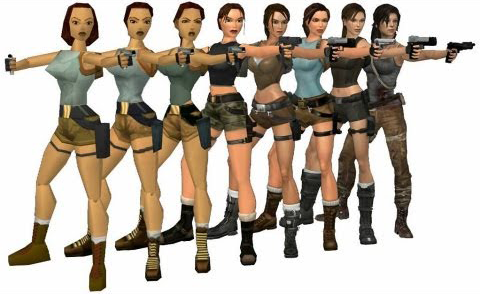
\includegraphics[width=1.0\textwidth]{images/tomb_raider_evolution.png}
    \caption{A Tomb Raider játéksorozat főszereplőjének evolúciója 1996 és 2008 között. Figyeljük meg, az évek alatt mennyivel részletesebb, a valóságos alakot egyre jobban visszaadó lett a karakter geometriája. }
\end{figure}

Önmagukban a háromszögeket meghatározó térbeli pozíciók még nem elégségesek. Ismernünk kell a felület tetszőleges pontjának irányultságát, amelyet egy, a felületből ,,kifelé'' álló, egység hosszúságú vektorral írunk le és felületi normálvektornak hívunk. Jelölése: \(\mathbf{n}\). Ezeket legegyszerűbben a háromszögeket alkotó pontokkal együtt tárolhatjuk, majd menet közben interpolálva őket kaphatjuk meg a háromszög által meghatározott felület tetszőleges pontján vett normálvektort.

\subsection{Az árnyalási egyenlet}

A számítógépes grafika egyik alaptételének tekinthető árnyalási egyenletet (\textit{rendering equation}) David Immel et al.~\cite{immel1986radiosity} és James Kajiya~\cite{kajiya1986rendering} írta le 1986-ban. Az egyenlet segítségével meghatározható a felület egy adott pontját elhagyó sugárzás a felület által kibocsátott ill. visszavert sugárzás összegének geometriai optika alapú közelítésével:

\[
L_{out}(\mathbf{x},\mathbf{v}) = L_{emit}(\mathbf{x},\mathbf{v}) + \int_\Omega f_r(\mathbf{x},\mathbf{l},\mathbf{v}) L_{in}(\mathbf{x},\mathbf{l}) (-\mathbf{l} \cdot \mathbf{n})\,\mathrm{d}\mathbf{l}
\]

\noindent
ahol a paraméterek:

\begin{itemize}[noitemsep]
\item \(\mathbf{x}\) a felület egy pontja,
\item \(\mathbf{v}\) a felület egy pontjából a nézeti pozícióba mutató normálvektor (nézeti vektor),
\item \(\mathbf{n}\) a korábban bevezetett felületi normálvektor,
\item \(\mathbf{l}\) pedig a felület egy pontjából a fényforrás felé mutató normálvektor.
\end{itemize}

\noindent
\textit{Megjegyzés: az eredeti egyenlet figyelembe veszi még az időt és a fény hullámhosszát is. Az egyenlet paraméterei az idő előrehaladtával ritkán változnak, és ebben az esetben is előre kiszámolhatóak, ezért gyakorlati alkalmazás esetén az időt állandónak tekinthetjük, amely így kiesik az egyenletből. Mivel számítógépes grafikánál RGB színtérben dolgozunk, és ennek 3 összetevőjét külön-külön számolhatjuk, így a hullámhossz paraméter is elhagyható. A továbbiakban ezért fény alatt a fény színét és erősségét értjük.}

A könnyebb érthetőség kedvéért bontsuk részekre az egyenletet. A bal oldalon szereplő \(L_{out}\) az eredmény: a felület egy pontjából érkező fényt határozza meg a nézeti vektor függvényében, később ez lesz a ténylegesen megjelenített színérték. A jobb oldal első tagja, \(L_{emit}\) a felület egy pontjából kisugárzott fényt adja meg. Ez az érték a gyakorlatban jellemzően 0, mert kevés emisszív anyag létezik, de pl. a fényforrások megjelenítéséhez szükség van rá.

A következő tag az integrál, amelyben az \(\Omega\) a felületi normálvektor körül vett félgömböt jelenti, ami az összes lehetséges \(\mathbf{l}\) vektort tartalmazza, amelyen integrálni kell a tartalmazott függvényeket. Mint később látni fogjuk, az integrálás lesz az egyik sarkalatos pontja az egyenlet gyakorlati alkalmazásának, ugyanis az integrálnak nem minden fényforrás esetén van analitikus megoldása --- ilyenkor közelítést fogunk alkalmazni. \(f_r\) az ún. kétirányú visszaverődési eloszlásfüggvény (bi-directional reflection distribution function, röviden BRDF), amelyről a következő alfejezetben lesz részletesen szó. \(L_{in}\) a felület adott pontjára \(-\mathbf{l}\) irányból beérkező fényt adja meg.

Fontos megjegyezni, hogy ez a fény nem csak direkt, hanem indirekt forrásból is érkezhet (pl. már valahol tükröződött fény, ld. globális/kép alapú megvilágítás).

Az utolsó tag, \(-\mathbf{l} \cdot \mathbf{n}\) a beérkező fény iránya és a felületi normálvektor által bezárt szög koszinusza alapján csökkenti a kisugárzott fény erősségét.

\subsection{Mikrofelület elmélet, diffúz és spekuláris tükröződés}

A fizikai alapú megjelenítés egyik alapköve a mikrofelület elmélet (\textit{microfacet theory}), ami szerint a nem tökéletesen sima felületeket úgy kell elképzelni, mintha sok apró, tökéletesen tükröző lapkából állnának. Ezen lapkák normálvektora a közelítő sima felület normálvektora körül oszlik el, és a kettő közötti eltérés mértékét hívjuk rücskösségnek vagy durvaságnak (\textit{roughness}), ami jellemzően egy \([0; 1]\) intervallumba eső érték (0 = tökéletesen sima, 1 = legdurvább).

Mielőtt a mikrofelületekkel tovább haladnánk, tisztáznunk kell, mit jelent a diffúz és a spekuláris tükröződés fogalma, ill. miben különbözik a kettő egymástól.

\begin{figure}[!ht]
    \centering
    \begin{subfigure}[b]{0.4\textwidth}
        \centering
        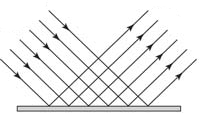
\includegraphics[width=\textwidth]{images/specular_reflection.png}
        \caption{Spekuláris visszaverődés}
    \end{subfigure}
    \hfill
    \begin{subfigure}[b]{0.4\textwidth}
        \centering
        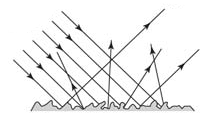
\includegraphics[width=\textwidth]{images/diffuse_reflection.png}
        \caption{Diffúz visszaverődés}
    \end{subfigure}

    \caption{A fénysugarak visszaverődése spekuláris és diffúz esetben.}
\end{figure}

Spekuláris tükröződésről akkor beszélünk, amikor egy sima felületre érkező fénysugarak mindegyike ugyanabba az irányba halad tovább a visszaverődés után. Diffúz tükröződés akkor történik, amikor egy durva felület különböző irányokba veri vissza, szórja szét a beérkező fénysugarakat. A mikrofelület elmélet segítségével ezt úgy képzelhetjük el, hogy a fénysugarak különböző irányultságú lapkákról verődnek vissza, így értelemszerűen különböző irányokba szóródnak szét.

Fontos megjegyezni, hogy spekuláris tükröződés nem csak tökéletesen sima felületek esetén fordul elő: ahogy a felület durvasága nő, úgy szóródnak egyre több irányba a fénysugarak, tehát annál kevésbé koncentráltan érik el a kamerát, ezáltal a ,,csillanás'' annál nagyobb méretű és halványabb lesz. A gyakorlatban a diffúz és a spekuláris tükröződést egymástól külön, különböző BRDF-fel számoljuk.

\subsection{A Blinn-Phong visszaverődési modell}

Mielőtt rátérnénk a fizikai alapú megjelenítés elméletére, fontos megismernünk a három dimenziós megjelenítésben a PBR előtt széles körben elterjedt, gyakorlatilag sztenderdnek nevezhető árnyalási modellt.

Bui Tuong Phong 1973-ban publikálta a később róla elnevezett tükröződési és árnyalási modelljeit~\cite{phong1975illumination}, amelyekre az utókor előszeretettel tekint együtt, egyszerűen a ,,Phong árnyalási modell'' elnevezést használva. A valódi, különálló Phong árnyalási modell lényegében a bevezetésben már említett felületi normálvektor interpolációt írja le: a vertexenként megadott normálvektorokból a felület bármely pontján interpolációval kiszámolható egy olyan normálvektor, amivel a tükröződést számolva a kapott felület az őt alkotó geometriához képest sokkal simábbnak tűnik. Lényegében ez az elgondolás alapozta meg a képpontonkénti megvilágítást (\textit{per-pixel lighting}), amely csak valamivel később, ennek számolására külön hardveres gyorsítással rendelkező grafikus kártyák megjelenésével vált elterjedtté és a korábban használt, vertexenként (és emiatt gyorsabban) számolható sík ill. Gouraud árnyaláshoz képest jelentős vizuális előrelépést jelentett.

\begin{figure}[!ht]
    \centering
    
\includegraphics[width=0.7\textwidth]{images/flat_gouraud_phong.png}
    \caption{Sík, Gouraud és Phong árnyalás összehasonlítása. }
\end{figure}

A Phong tükröződési (vagy megvilágítási) modell egy tapasztalati modell egy felület pontjainak lokális megvilágításának kiszámítására. A felület \(p\) pontjából visszavert fény a Phong modell szerint a következőképpen számolható:

\[
L_{p} = k_a i_a + \sum_{m \in \textrm{lights}} {\left( k_d (L_m \cdot N) i_{m,d} + k_s(R_m \cdot V)^\alpha i_{m,s} \right)}
\]

\noindent
ahol a jelenetben szereplő összes anyagmodellre definiálva van

\begin{itemize}[noitemsep]
\item \(k_a\) ambiens tükröződési állandó,
\item \(k_s\) spekuláris tükröződési állandó,
\item \(k_d\) diffúz tükröződési állandó,
\item \(\alpha\) ragyogási állandó, amely sima felületeken nagyobb, és ilyenkor kis, koncentrált csillanást eredményez.
\end{itemize}

A tükröződési állandók a beérkező fénynek az anyag felszínéről történő tükröződésének mértékét adják meg. Az ambiens, vagy ,,elérhető'' fény a jelenet leképezése során implicit létező (napfény, holdfény, villámlás) megvilágítást jelenti.

\vspace{12pt}
\noindent
Ezen kívül

\begin{itemize}[noitemsep]
\item \(lights\) a fényforrások halmaza,
\item \(L_m\) a felület \(p\) pontjából az adott fényforrás irányába mutató vektor,
\item \(N\) a felületi normálvektor,
\item \(R_m\) a tükröződési vektor, és
\item \(V\) a nézeti vektor.
\end{itemize}

\noindent
\textit{Megjegyzés: az \(L_m\), \(N\), \(R_m\) és \(V\) vektorok egység hosszúságúak.}

\vspace{12pt}

A Blinn-Phong tükröződési modell~\cite{blinn1977models} a Phong modell James F. Blinn által módosított változata: az \(R_m \cdot V\) skalárszorzat helyett \(N \cdot H\)-t használ, ahol a \(H\) egy ún. félszög vektor (\textit{half-angle vector}) a nézeti és a fényforrás irányába mutató vektorok között:

\[
H = \frac{ L + V }{ \| L + V \| }
\]

Ennek előnye megjelenésének idején elsősorban az volt, hogy a \(H\) vektort gyorsabban ki lehetett számolni, mint az \(R\)-t. Végül ez a modell vált a de-facto sztenderd árnyalási modellé, mind az OpenGL, mind a DirectX fix-funkciós csővezetéke ezt a modellt használja. További előnye az eredeti Phong modellel szemben, hogy sík felületen történő tükröződéskor kis szögű vézeti vektor esetén a csillanás ,,megnyúlik'', elliptikus alakot vesz fel, így jobban közelítve a valóságban tapasztalható jelenséget (szemben a Phong modellel, amely mindig kör alakú csillanást eredményez), továbbá a \(H\) vektorral történő számolás a később tárgyalt, fizikai alapú megjelenítést megalapozó mikrofelületi modellhez hasonlatos.

\begin{figure}[!ht]
    \centering
    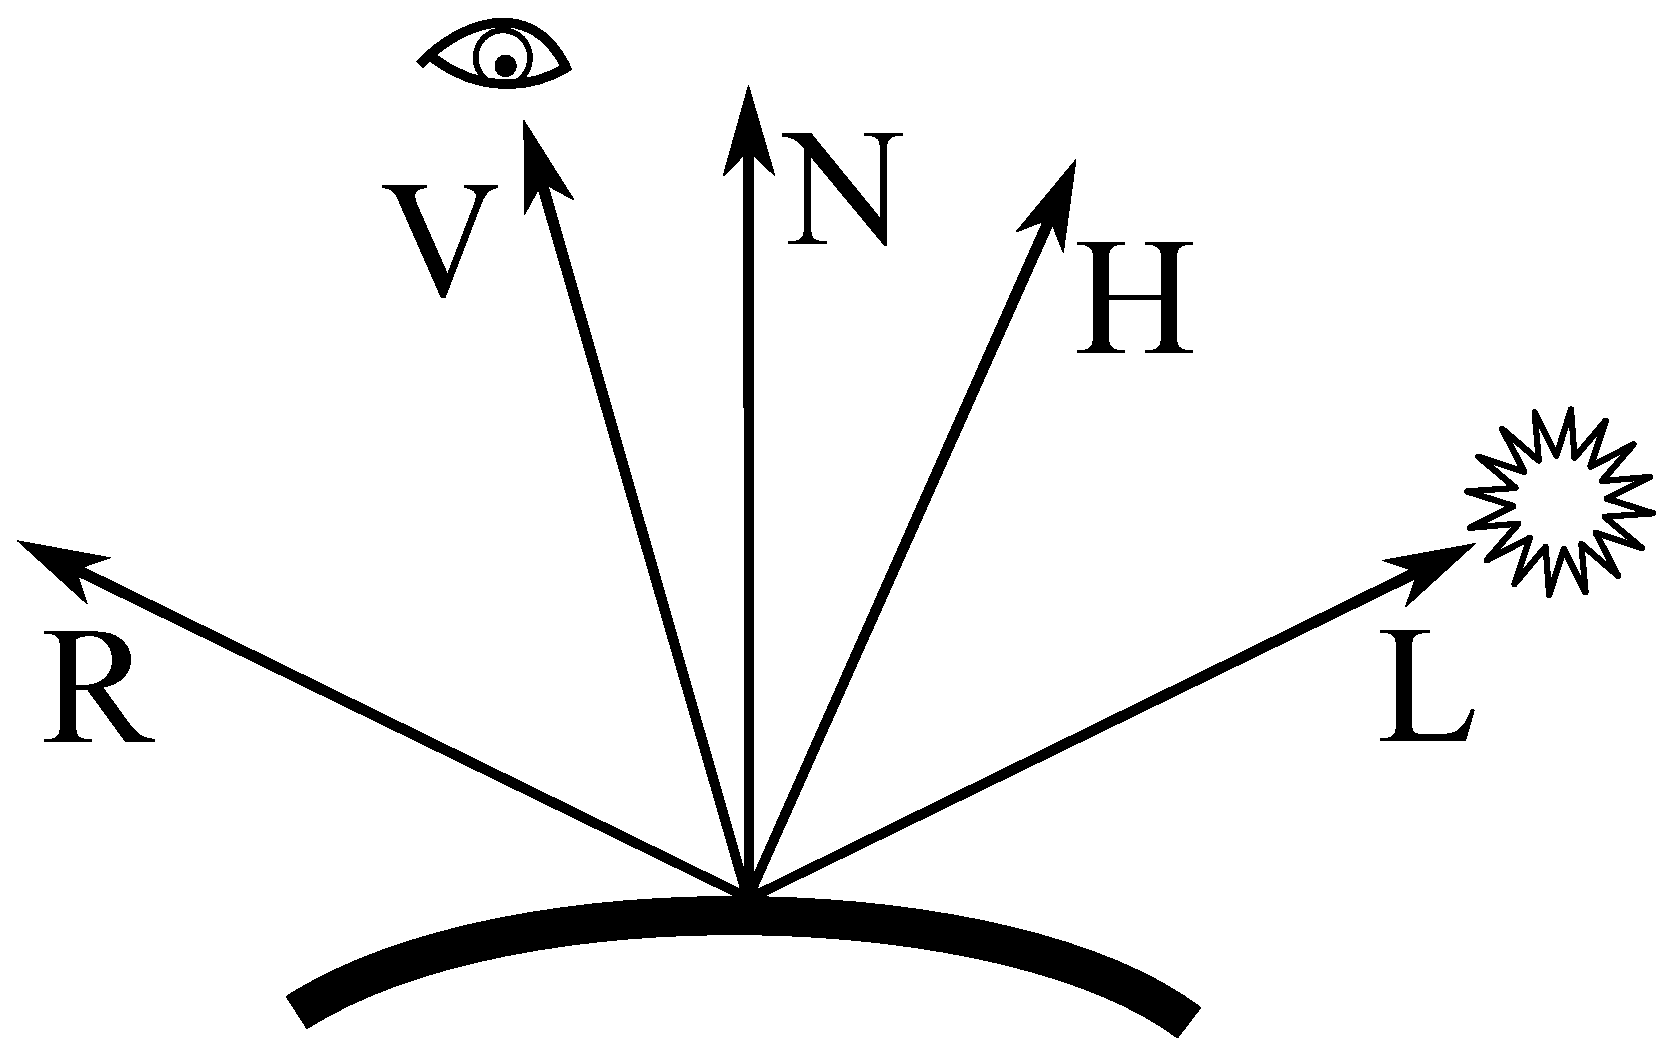
\includegraphics[width=0.4\textwidth]{images/blinn_vectors.eps}
    \caption{A Phong és a Blinn-Phong visszaverődési modell vektorai.}
\end{figure}

A gyakorlatban a \(k\) anyagparaméterekre színvektorokat használunk, így lényegében egyszerre számoljuk a vörös, zöld és kék fények tükröződését. A modell definíciójából látható, hogy az anyagparaméterek mindegyike tapasztalati alapon kitalált, nincs egzakt fizikai mértékegységük, hiszen nem konkrét fizikai modellen alapulnak. Az anyag által meghatározott ambiens tükröződési érték is furcsának hat, hiszen logikusan gondolkozva ezt a megvilágítást a jelenet alapján kellene kiszámítani, itt mégis az anyagtulajdonságok között szerepel. A Blinn-Phong modell egyik nagy hátránya is ebből fakad: egy adott megvilágítás mellett elkészített, szemmel jónak ítélt anyagmodellt más megvilágítás alá helyezve ,,elromlik'' a megjelenítés, a fix és fizikai alapot nélkülöző paraméterek miatt.

\subsection{Matematikai és fizikai alapfogalmak}
\label{subsec:matbase}

A térszög (\textit{solid angle}, jelölése: \(\Omega\)) egy objektum egy ponttal bezárt kétdimenziós szöge háromdimenziós térben. Mértékegységét \textit{szteradiánnak} nevezzük és \(sr\)-rel jelöljük.

\begin{figure}[!ht]
    \centering
    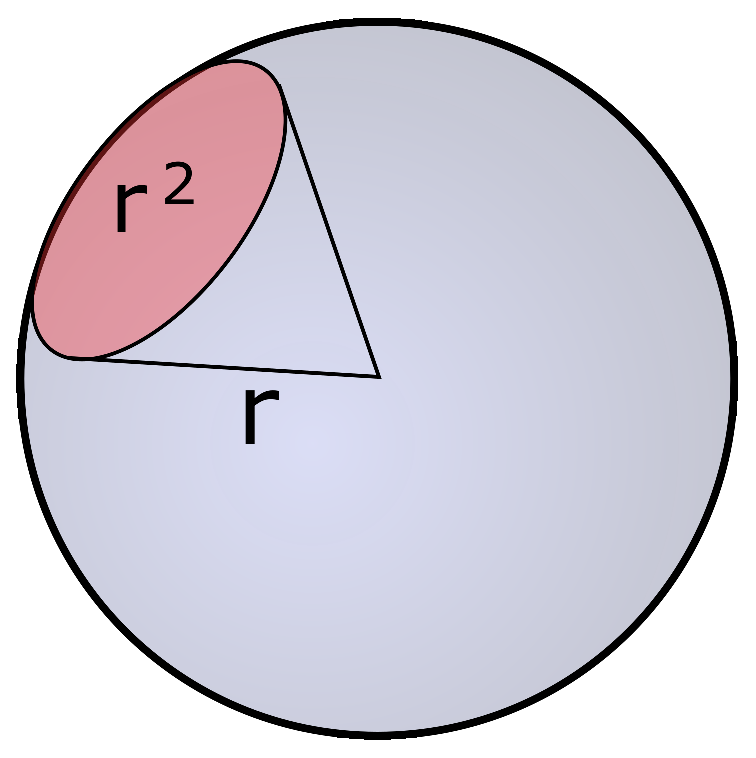
\includegraphics[width=0.3\textwidth]{images/steradian.eps}
    \caption{Bármely terület egy gömb felszínén, ami megegyezik sugarának négyzetével, a gömb középpontjából nézve pontosan egy szteradiánt zár be.}
\end{figure}

A radiometria az elektromágneses sugárzás (esetünkben a látható fény) mérésével foglalkozik. A következő definíciókban a könnyebb érthetőséget és a későbbi gyakorlati megvalósítást szem előtt tartva nem mindig az eredeti, fizikai definíciókban szereplő jelöléseket, hanem a korábban bevezetett vektortípusokat használtam.

\begin{itemize}[noitemsep]
\item \(\phi\): sugárzási teljesítmény (\textit{radiant flux}),
\item \(E\): besugárzás (\textit{irradiance}),
\item \(I\): sugárerősség (\textit{radiant intensity}),
\item \(L\): sugársűrűség (\textit{radiance}).
\end{itemize}

A sugárzási teljesítmény egy tartományon egységnyi idő alatt átáramló sugárzási energiát jelöli és Wattban (W) mérjük. A besugárzás az egységnyi területre beérkező sugárzási teljesítmény adja meg. Mértékegysége \(W \over m^2\), és a következőképpen számolható:

\[
E = { { d\phi } \over { dA } }
\]

\noindent
ahol \(d\) a parciális derivált szimbóluma, \(\phi\) a sugárzási teljesítmény és \(A\) a terület.

\vspace{12pt}

A sugárerősség az egységnyi térszögben terjedő sugárzási teljesítményt adja meg, mértékegysége \(W \over {sr}\), definíciója pedig:

\[
I = { { d\phi } \over { d\omega } }
\]

\noindent
ahol \(\omega\) infinitezimális térszög.

\vspace{12pt}

A radiancia az egységnyi vetített területre egységnyi térszögben beérkező, visszavert, vagy emittált sugárzási teljesítményt határozza meg. Ez a legfontosabb fogalom a felsoroltak közül, ugyanis a megjelenítés során ezt az értéket, azaz a megjelenítendő felület egy adott pontját adott irányban elhagyó sugárzást kell kiszámoljuk. Mértékegysége \(W \over {m^2sr}\), és a következőképpen definiáljuk:

\[
L(\mathbf{v}) = { { d^2\phi } \over { dA cos\theta d\mathbf{v} } }
\]

\noindent
ahol \(\theta\) a felületi normálvektor és a nézeti vektor által bezárt szög.

\vspace{12pt}

\noindent
A besugárzás kiszámítására a későbbiekben pedig a következő képlet ad lehetőséget:

\[
dE(\mathbf{l}) = d { {d\phi} \over {dA} } (\mathbf{l}) = L_{in}(\mathbf{l}) cos\theta_l d\mathbf{l}
\]

\subsection{A kétirányú visszaverődési eloszlásfüggvény}

A kétirányú visszaverődési eloszlásfüggvényt, azaz BRDF-et Fred Nicodemus definiálta először~\cite{nicodemus1965directional}, és arra a feltevésre épül, hogy a nézeti irányba visszavert fény arányos a fényforrás által besugárzott fénnyel. Ezek alapján definíciója a következő:

\[
f_r(\mathbf{l}, \mathbf{v}) = { { dL_{out}(\mathbf{v}) } \over {dE(\mathbf{l})} }
\]

A BRDF egyik előnye, hogy fizikailag mérhető: az interneten található MERL adatbázis~\cite{merl_database} 100 különböző anyag visszaverődési függvényét tartalmazza.

\vspace{12pt}

\noindent
Tulajdonságai:

\begin{itemize}[noitemsep]
\item pozitív: \(f_r(\mathbf{l},\mathbf{v}) \geq 0\)
\item szimmetrikus: \(f_r(\mathbf{l},\mathbf{v}) = f_r(\mathbf{v},\mathbf{l})\)
\item teljesíti az energiamegmaradás törvényét: \(\int_\Omega f_r(\mathbf{l},\mathbf{v}) (-\mathbf{l} \cdot \mathbf{n})\,\mathrm{d}\mathbf{l} \leq 1\)
\end{itemize}

A Blinn-Phong modellhez hasonlóan a fizikai alapú megjelenítés során is külön számoljuk a diffúz és a spekuláris megvilágítást, emiatt minden megvilágítási típushoz két megfelelő, diffúz és spekuláris BRDF-et kell találjunk.

A valósidejű grafikában minimális számításigénye miatt leggyakrabban használt diffúz BRDF a Lambert-féle tükröződésen alapuló \textit{Lambert BRDF}, amely a következőképpen definiált:

\[
f_{Lambert}(\mathbf{l}, \mathbf{v}) = { c_{diff} \over \pi }
\]

ahol \(c_{diff}\) az anyag diffúz visszaverődési aránya, gyakorlati megvalósítás során a színe. A \(\pi\)-vel való osztás az energiamegmaradás miatt szükséges, ugyanis:

\[
\int_\Omega { (-\mathbf{l} \cdot \mathbf{n}) \mathrm{d}\mathbf{l} } = \int_\Omega { cos(\omega_l) \mathrm{d}\mathbf{l} } = \pi
\]

Tehát \(\pi\) kiesik, \(c_{diff}\) állandó integrálja pedig értelemszerűen már teljesíti az energiamegmaradás törvényét.

A Lambert-féle tükröződés Johann Heinrich Lambert nevéhez fűződik, aki 1760-ban írta le ezt a jelenséget Photometria c. könyvében~\cite{klett1760ih}. A Lambert-féle tükröződés szerint egy ideális diffúzan tükröző, azaz matt felület (Lambert felület) a nézeti pozíciótól függetlenül ugyanolyan fényesnek látszik, vagyis teljesíti Lambert koszinusz törvényét, ami szerint az ilyen felületek megfigyelhető fényessége közvetlenül arányos a fényforrásba mutató vektor \(\mathbf{l}\) és a felületi normálvektor \(\mathbf{n}\) által bezárt szög koszinuszával.

A Lambert BRDF jól használható diffúz felületek megvilágításának közelítésére, azonban tudnunk kell, hogy nagyon kevés tökéletes Lambert felület létezik, így nem-valósidejű megjelenítésnél, ahol nem ennyire hangsúlyos tényező a futásidő, érdemes más, a valóságban gyakran előforduló rücskös felületek megjelenését jobban közelítő BRDF-et választani. Két lehetséges alternatíva a Disney által kifejlesztett Burley~\cite{burley2012physically} illetve az Oren-Nayar visszaverődési modell~\cite{oren1994generalization}, amely a felület rücskösségét is figyelembe veszi.

\begin{figure}[!ht]
    \centering
    \begin{subfigure}[b]{0.25\textwidth}
        %\right
        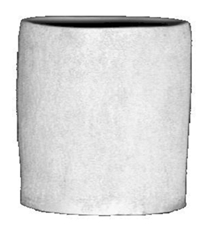
\includegraphics[width=\textwidth]{images/vase_a.png}
        \caption{A valódi váza}
    \end{subfigure}
    \hfill
    \begin{subfigure}[b]{0.25\textwidth}
        %\centering
        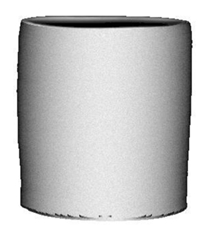
\includegraphics[width=\textwidth]{images/vase_b.png}
        \caption{Phong}
    \end{subfigure}
    \hfill
    \begin{subfigure}[b]{0.25\textwidth}
        %\left
        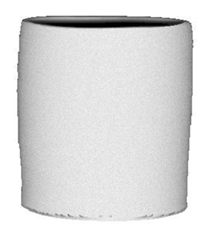
\includegraphics[width=\textwidth]{images/vase_c.png}
        \caption{Oren-Nayar}
    \end{subfigure}

    \caption{Egy valódi váza és annak számítógéppel megjelenített változatai különböző diffúz modellekkel.}
\end{figure}

A spekuláris BRDF-re, azaz a visszaverődő fény által létrehozott csillanás kiszámolására rengeteg modell létezik. Ebből egyet már ismerünk, ami a Blinn-Phong visszaverődési modellben található spekuláris komponens kiszámítására vonatkozó részlet. A valós idejű fizikai alapú megjelenítők túlnyomó többsége azonban az ún. Cook-Torrance modellt használja, amit R. Cook és K. Torrance dolgozott ki 1981-ben~\cite{cook1981reflectance}.

\[
f_{CookTorrance}(\mathbf{l}, \mathbf{v}) = { {D(\mathbf{h}) F(\mathbf{l}, \mathbf{h}) G(\mathbf{l}, \mathbf{v}, \mathbf{h})} \over {4(\mathbf{n} \cdot \mathbf{l})(\mathbf{n} \cdot \mathbf{v})} }
\]

\vspace{12pt}

\noindent
ahol

\begin{itemize}[noitemsep]
\item \(D(\mathbf{h})\) a mikrofelület normálvektorainak eloszlásfüggvénye,
\item \(F(\mathbf{l}, \mathbf{h})\) a Fresnel tényező, és
\item \(G(\mathbf{l}, \mathbf{v}, \mathbf{h})\) a geometriai halványító tényező.
\end{itemize}

Nézzük először a Fresnel-tényezőt. Az Augustin-Jean Fresnel által kikövetkeztetett Fresnel egyenletek a fény viselkedését írják le két különböző törésmutatójú közeg közti áthaladása során: ilyenkor mind tükröződés, mind fénytörés előfordulhat. A Fresnel egyenletek leírják, hogy a fény mekkora része tükröződik és mekkora része törik meg ilyenkor. A fény tükröződése, amit az egyenletek megjósolnak Fresnel tükröződésként is ismert. Mivel a Fresnel egyenletek túl bonyolultak ahhoz, hogy valósidőben számoljunk velük, ezért valósidejű megjelenítőknél a Christophe Schlick által kifejlesztett közelítést használják a spekuláris tükröződés Fresnel tényezőjének kiszámítására.~\cite{schlick1994inexpensive}

\[
F_{Schlick}(\mathbf{l}, \mathbf{h}) = F_0 + (1 - F_0)(1 - \mathbf{l} \cdot \mathbf{h})^5
\]

ahol \(F_0\) a tükröződési együttható a felületi normálvektorral párhuzamos beérkező fényekre, és a következőképpen számolható:

\[
F_0 = \left( {n_1 - n_2} \over {n_1 + n_2} \right)^2
\]

Itt \(n_1\) és \(n_2\) a két közeg törésmutatója. Mivel számítógépes grafikában az egyik közeg szinte mindig a levegő, ezért \(n_1\) 1-gyel helyettesíthető. A szigetelő anyagok többségének törésmutatója 1,5 körül mozog, ezért ezekre az anyagokra \(F_0\)-nak 0,04 jó közelítése. Fémeknél \(F_0\) a fém színével ekvivalens.

Az eredeti Cook-Torrance modell \(D\)-re a Beckmann eloszlást~\cite{beckmann1987scattering} használja, amely egy fizikai alapú modell a mikrofelületi eloszlásra.

\[
D_{Beckmann}(\mathbf{n}, \mathbf{h}) = { { e^{ -tan(\alpha)^2 \over m^2 } } \over { \pi m^2 cos(\alpha)^4 } }
\]

\noindent
ahol

\begin{itemize}[noitemsep]
\item \(\alpha = arccos(\mathbf{n} \cdot \mathbf{h})\), és
\item \(m\) a mikrofelület lapkáinak négyzetes közepének meredeksége (a felület rücskössége).
\end{itemize}

Ugyan a képlet még egyszerűsíthető, ezzel együtt is szemmel láthatóan nagy a számításigénye. Ezért a gyakorlatban az ún. GGX eloszlásfüggvényt~\cite{walter2007microfacet} használjuk:

\[
D_{GGX}(\mathbf{n}, \mathbf{h}) = { \alpha \over { \pi ((\mathbf{n} \cdot \mathbf{h})^2 (\alpha^2 - 1) + 1)^2 } }
\]

\noindent
ahol \(\alpha = {roughness}^2\) (roughness = rücskösség).

\section{Gyakorlati megvalósítás}

Egy háromdimenziós megjelenítő fejlesztésekor mind programozási nyelv, mind megjelenítő API szempontjából több választási lehetőség áll előttünk. Valósidejű megjelenítőről lévén szó azonban nagyon fontos, hogy a választott programozási környezet járulékos lassító tényezői (pl. menedzselt nyelvek --- Java, C\# stb. --- esetén a futtatókörnyezet, ill. szemétgyűjtő futási sebességre és felhasznált memóriára vonatkozó negatív hatása) minél kevésbé befolyásolja a program futását. Ezért --- követve az iparág nagy szereplőit --- választásom a C++ programozási nyelvre esett. A C++ fordított nyelv, azaz forráskódunkból a processzor által közvetlenül végrehajtható, a fordító által erősen optimalizált gépi kód készül. Ennek egyik hátránya, hogy processzor architektúrához és operációs rendszerhez kötődő futtatható állományt kapunk, azaz minden kívánt platformra külön le kell fordítsuk forráskódunkat --- ellentétben pl. a Java-val, amely platformfüggetlen bájtkódot állít elő, és azt a gépre előre telepített, platformspecifikus futtatókörnyezet hajtja végre. Előnye viszont, hogy minden platformra külön optimalizált futtathatót készíthetünk, ami valósidejű megjelenítésnél a futási sebesség szempontjából fontos lehet. A C++ eléggé alacsonyszintű ahhoz, hogy minden teljesítmény szempontjából számító befolyásoló tényezőt (pl. memóriafoglalás, annak pontos ideje és mérete) a kezünkben tarthassunk, de közben eléggé magasszintű ahhoz, hogy az objektum-orientált programozást lehetővé tevő nyelvi eszközei és standard könyvtára (\textit{standard template library, STL}) segítségével hatékonyan írhassunk benne összetett programokat.

A megjelenítő fejlesztése során igyekeztem minél jobban igénybe venni az új C++ szabványok (C++11, C++14) által bevezetett szintaktikai és STL-t érintő újdonságokat (okos mutatók, új tömb tároló, automatikus típuslevezetés, stb.), illetve a ,,modern C++'' meghatározó eszközeit (kivételkezelés, RAII), amelyek segítségével egy átlátható, könnyedén bővíthető, robosztus kódbázis született.

A C++ projekt definiálására és lefordításának megkönnyítése érdekében a CMake build rendszert használtam. A CMake segítségével platformfüggetlen módon definiálhatunk egy C vagy C++ projektet: néhány alapvető adaton kívül meg kell adnunk a forrásfájlokat és a függőségeket, majd ebből a CMake legenerálja a szükséges fájlokat a kívánt natív build rendszerrel történő fordításhoz. A fejlesztés elsősorban Windows operációs rendszeren, Visual Studio fejlesztőkörnyezetben folyt, de mind a forráskód megírásánál, mind a build rendszer kiválasztásánál figyeltem arra, hogy a program a használt könyvtárak által támogatott platformok mindegyikére könnyedén lefordítható legyen.

Az asztali számítógépeken a két legelterjedtebb grafikus API a DirectX és az OpenGL. Okostelefonokon az OpenGL speciális, kisebb tudású, áramvonalasított változata, az OpenGL ES az egyeduralkodó API. A konzolokon jellemzően erősen a célhardverre specializált alacsonyszintű programozási felületek állnak rendelkezésre, amelyek elérése külön feltételekhez kötött, így ezekről kevés információnk áll rendelkezésre. A két rivális asztali API közül azért az OpenGL-re esett a választásom, mert volt már vele tapasztalatom, és mert keresztplatformos, míg a DirectX csak Microsoft Windows rendszereken érhető el.

Habár az OpenGL a 3-as főverzióval komoly ráncfelvarrást kapott, felépítésében továbbra is egy erősen egy szálon futó állapotgép maradt. A modern GPU-k azonban architekturálisan már tovább fejlődtek ennél: az új, alacsonyszintű API-k már hatékonyan kezelik a több szálról érkező parancsokat, ami az OpenGL-ben csak költséges módon (\textit{context switch}) megoldható. Ezzel elsősorban a kirajzolási hívásszám-limitált jelenetekben (pl. részecskerendszerek kirajzolása) érhető el az OpenGL-nél jóval magasabb teljesítmény.

További lassító tényező az OpenGL magasszintűsége, ami a fejlesztőknek ugyan valamekkora kényelmet és időbeli nyereséget jelenthet, azonban egyrészt emiatt a grafikus kártya meghajtóprogramjának kell sok olyan dolgot általános módon implementálnia (pl. biztonságos videomemória-kezelés), amit sok esetben a fejlesztők a saját igényeiket és céljaikat ismerve optimálisabban is meg tudnának írni, másrészt a meghajtóprogram sok ellenőrzést is végrehajt a kapott inputokon, ami processzor oldalon felesleges többletterhelést jelenthet.

A szakdolgozat írásának idején megjelent új API-k --- DirectX 12, Vulkan (lényegében az OpenGL revolúciós folytatása), Metal (Apple rendszereken) --- ezeket a problémákat küszöbölik ki: alacsony szintűek, explicitek és erősen támogatják a többszálúságot.

\subsection{A felhasznált nyílt forráskódú könyvtárak bemutatása}

Munkám során a fejlesztést megkönnyítendő, és a programozás egyik alapvető tételét, az újrafelhasználást figyelembe véve a fizikai megjelenítéshez szorosan nem kapcsolódó részeket nyílt forráskódú könyvtárak segítségével valósítottam meg. A megjelenítő ablakának ill. az OpenGL környezet létrehozását, továbbá az ehhez kapcsolódó eseménykezelést (egérmozgás, billentyűzet kezelés, ablakesemények) a C-ben írt, keresztplatformos GLFW könyvtár végzi. Ahhoz, hogy az OpenGL bővítményeit használni tudjam, a Python alapú GLAD OpenGL függvénymutató-betöltővel generáltam C forrásfájlt, amelyben a legújabb, 4.5-ös OpenGL verzióig az összes függvénymutató, ill. az ezeket inicializáló mechanizmus megtalálható. Grafikus alkalmazásoknál, kiváltképp három dimenzióban elkerülhetetlen a lineáris algebra használata. Ehhez a népszerű GLM fejléc alapú C++ sablonkönyvtárat választottam, amely az OpenGL árnyalónyelve, a GLSL mintájára készült, és a legfontosabb lineáris algebrai konstrukciók (egész és lebegőpontos vektorok, mátrixok, kvaterniók) mellett többek közt az ezek között definiált műveletek megvalósítását és sok hasznos segédfüggvényt (pl. vetítési, nézeti mátrix létrehozása) is tartalmaz. A megjelenítő elsődleges bemenetét képező 3D-s Wavefront OBJ formátumú modellek betöltését a tinyobjloader C++ könyvtár végzi, amely a hozzájuk csatolt anyagtulajdonság-leíró fájlokat (.mtl kiterjesztéssel) is feldolgozza. A felhasználói felület megjelenítéséért és kezeléséért az OpenGL alapú NanoGUI könyvtár felel, amely a NanoVG (szintén OpenGL-alapú) közvetlen módú vektorgrafikus rajzoló könyvtárra épül. Ezen könyvtárak mindegyike nyílt forráskódú és folyamatos fejlesztés alatt áll, így probléma esetén a szükséges módosításokat végre tudtam hajtani rajtuk, ami --- mindamellett, hogy segítségükkel a fizikai megjelenítés konkrét implementációjára koncentrálhattam --- nagy segítséget jelentett a fejlesztés során.

\subsection{A megjelenítő felépítése}

TODO: ábra a felépítésről

Ugyan az OpenGL egy meglehetősen magas szintű grafikus programozási felület, a kódismétlés elkerülése és az átláthatóság könnyítése érdekében több egyszerű burkoló (\textit{wrapper}) objektumot is létrehoztam a leggyakrabban használt OpenGL objektumok köré. Ezek a Shader, Program, VertexArray, VertexBuffer, FrameBuffer és Texture (Texture2D, TextureArray és TextureCubeMap) osztályok.

A program belépési pontja, a main() függvény először létrehoz egy Settings objektumot a kapott parancssori argumentumok alapján, majd ennek segítségével létrehoz egy Renderer objektumot, amin meghívja a Renderer osztály egyetlen metódusát, a run()-t. Mivel a megjelenítő a végzetes hibák jelzésére kivételkezelést használ, ezért az egész program egy try/catch blokkban fut, így a korábban el nem kapott kivételek legkésőbb a main()-ben elfogásra kerülnek, a bennük tárolt hibaüzenet kiíródik és a program kilép. Ilyen végzetes hiba például az, ha egy árnyalóprogram lefordítása valamiért nem sikerül.

A Renderer konstruktora a kapott beállítások alapján létrehoz egy OpenGL ablakot a Window osztály segítségével, ami tulajdonképpen egy GLFW ablakot kezel objektum-orientált módon. Ezután létrehozza a két beépített fényt, majd a felhasználói felület inicializálása következik. Ekkor már van OpenGL kontextusunk, ezért a modell és vetítési mátrixok beállítása után létrehozza a szükséges árnyalóprogramokat és képpont puffereket. Végül pedig létrehozza az alapértelmezett Mesh illetve Skybox objektumokat.

A Renderer run() metódusa tartalmazza a program főciklusát, ami a program folyamatos futását okozza. Ebben a ciklusban a következő lépések történnek:

\begin{figure}[!ht]
    \centering
    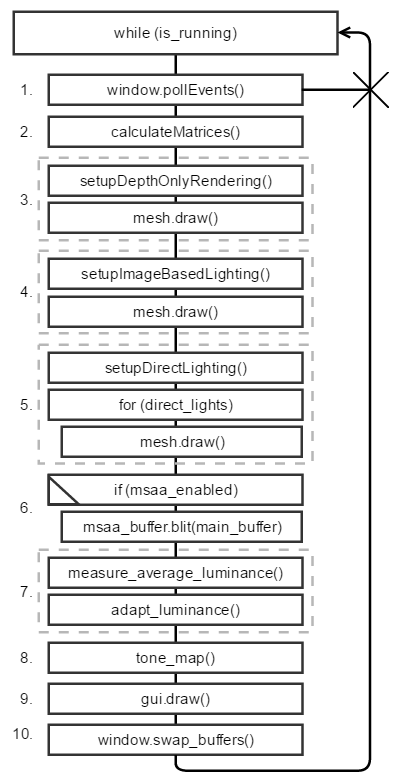
\includegraphics[width=0.45\textwidth]{images/main_loop.png}
    \caption{A főciklus szekvenciadiagramja}
\end{figure}

\begin{enumerate}[noitemsep]
  \item operációs rendszer által küldött események feldolgozása (a GLFW segítségével)
  \item a megjelenítés során használt mátrixok (modell, nézeti, vetítési) illetve ezek különféle kombinációinak kiszámolása
  \item egy előlépésben a modell kirajzolása, de csak a mélységi pufferbe
  \item a modell kirajzolása kép alapú megvilágítással
  \item a modell kirajzolása pont vagy zseblámpa fényenként egyszer, bekapcsolt additív színkeverés mellett
  \item ha be volt kapcsolva az élsimítás, akkor az MSAA puffer másolása a fő képpont pufferbe
  \item átlagos fénysűrűség mérése, majd az ehhez történő adaptáció
  \item színleképezés a választott operátor használatával (ennek során kerül a kép a fő képpont pufferből az ablak alapértelmezett pufferébe)
  \item a felhasználói felület kirajzolása
  \item a kettős pufferelés során használt elő- és háttérpufferek megcserélése, az elkészült képkocka megjelenítése
\end{enumerate}

A főciklust megszakítani, és ezzel a program futását leállítani a megjelenítő ablakának bezárásával lehet.

\subsection{Anyagok és modellek leírása}

Ahogyan az elméleti alapozás bevezetőjében elhangzott, a valósidejű megjelenítők térbeli háromszögekből építik fel a kirajzolt 3D-s modelleket, hiszen a GPU-k is ezeken dolgoznak hardver szinten. Ahhoz, hogy ezeket a modelleket ki tudjuk rajzolni, az őket leíró geometriát előbb fel kell tölteni a videomemóriába a használt grafikus API segítségével. Ezeket a geometriákat ún. vertexekkel adjuk meg. Egy vertex egy térbeli ponthoz rendelt attribútumok csoportja, minimálisan a pont pozícióját megadó vektort tartalmazza, de a háromszögháló adott pontjához tartozó normálvektort és textúrakoordinátát is a vertexben szokás tárolni. Értelemszerűen három vertex határoz meg egy térbeli háromszöget.

Textúrakoordinátákra (szokás UV-nak is nevezni őket) akkor van szükség, ha a modellt textúrázni szeretnénk, azaz egy kétdimenziós képet rá szeretnénk feszíteni kirajzolás során a háromszöghálóra. Ilyenkor egy jellemzően négyzetes textúrát használunk, amelynek pontjaira egy \([0; 1]\) intervallumba eső koordinátával hivatkozunk, és ezeket tároljuk el a vertexekben. Lehetőség van ezen az intervallumon kívül eső koordináták használatára is, ilyenkor a textúra létrehozásánál beállított \textit{wrap} (,,burkolási'') módtól függően többszöröződik, tükröződik, stb. a textúra a kívül eső koordinátákon. Egyszerű geometriáknál (pl. síkbeli négyzet) kézzel is megadhatóak ezek a koordináták, bonyolultabb modellek esetén azonban a 3D művészek, modellezők készítik el a textúrákat és állítják be pontosan a koordinátákat a használt modellező szoftver (Blender, Autodesk 3ds Max, Maya, stb.) segítségével.

Ezeket a vertexhalmazokat ,,beégethetjük'' a kódba (ld. skybox kocka), vagy betölthetjük külső forrásból a program futása közben. Számos különböző modellformátum létezik, az elkészített megjelenítő ezek közül a Wavefront által kifejlesztett OBJ formátumú modellek betöltésére képes a tinyobjloader könyvtár segítségével. Egy OBJ fájlban a modellt alkotó háromszögháló csúcspontjainak pozíciói (illetve opcionálisan normálvektorok és textúrakoordináták) szöveges adatként szerepelnek. Ennek előnye, hogy akár kézzel, egy szövegszerkesztővel is módosíthatóak ezek az adatok, hátránya viszont, hogy a beolvasást jelentősen lassítja a szövegből lebegőpontos számmá konvertálás folyamata. Egy OBJ fájlban lehetőség van a modellt kisebb részegységekre, alakzatokra (\textit{shape}) bontani. A megjelenítő külön-külön, egymás után rajzolja ki ezeket az alakzatokat, így lehetőség van a megjelenítésüket egyenként ki/bekapcsolni.

Az OBJ fájlok mellé opcionálisan tartozhatnak MTL (material) fájlok is, amelyek a felhasznált anyagok tulajdonságait írják le. Habár az OBJ formátum lehetőséget ad rá, hogy akár háromszög-szinten különböző anyagokat használjunk, az egyszerűség kedvéért a megjelenítő csak az alakzatokhoz tud külön anyagot rendelni. Az eredeti fájlformátumban az anyagtulajdonságok elsősorban a Blinn-Phong árnyalási modell paraméterei (ambiens, diffúz, spekuláris tükröződési állandó, stb.), azonban a formátum egyszerű felépítése miatt könnyű saját paramétereket hozzáadni a leíráshoz. Ezért a mellékelt példamodellek anyagleíróiba bekerült két egyedi tulajdonság, a map\_Roughness és a map\_Metalness, amelyek a rücskösségi ill. fémességi textúratérkép (\textit{texture map}) elérhetőségeit tartalmazzák.

De mi is pontosan a textúra/textúratérkép? Tegyük fel, hogy egy téglafalat szeretnénk számítógéppel megjeleníteni. Adja magát az ötlet, hogy készítsünk egy olyan háromszöghálót, ami a maltertől kezdve a téglák repedésein át az egyenetlen felületekig mindent nagy részletességgel tartalmaz, majd az egyes háromszögeknek csak egy színt adva (tégla: vörös, malter: szürke) jelenítsük meg ezt a geometriát. Az elméletben jó ötlet a gyakorlatban kevésbé működőképes: egy ilyen részletességű háromszögháló megjelenítése, pláne valósidőben túl költséges a mai hardverek számára. Csinálhatjuk viszont a következőt: készítsünk egy egyszerű téglalap geometriát (maximum 6 vertexből megoldható), fotózzunk le merőlegesen egy téglafalat, majd az elkészült képet egyszerűen feszítsük rá geometriánkra a textúrakoordináták segítségével.

A textúrázás alapvető lényege tehát egy valódi felület élethű megjelenítéséhez túl alacsony felbontású geometria optikai részletességének látszólagos növelése egy ráfeszített kép segítségével. Jó minőségű textúra esetén az így megjelenített téglafal igazán élethű, de csak ha szemből nézünk rá. Minél kisebb szögben nézünk a téglalapunkra, annál szembetűnőbb lesz, hogy csak egy sík felületet látunk, ,,hiányzik'' az igazi téglafal domborúsága. Tudnunk kell azonban, hogy egy textúrában nem csak a felület színeit tárolhatjuk el. Ha például tudjuk (vagy modellezőprogram segítségével előállítjuk) egy felület minden egyes pontjának felületi normálvektorát, akkor ezeket a normálvektorokat kis átalakítás után eltárolhatjuk egy hagyományos RGB textúrában, amit normáltérképnek hívnak. Ha a kirajzolás során ebből a textúrából olvassuk ki az adott pont normálvektorát, akkor az árnyalás már emlékeztetni fog a valódi téglafalra, a csillanások és árnyékok növelni fogják valóságérzetünket.

\begin{figure}[!ht]
    \centering
    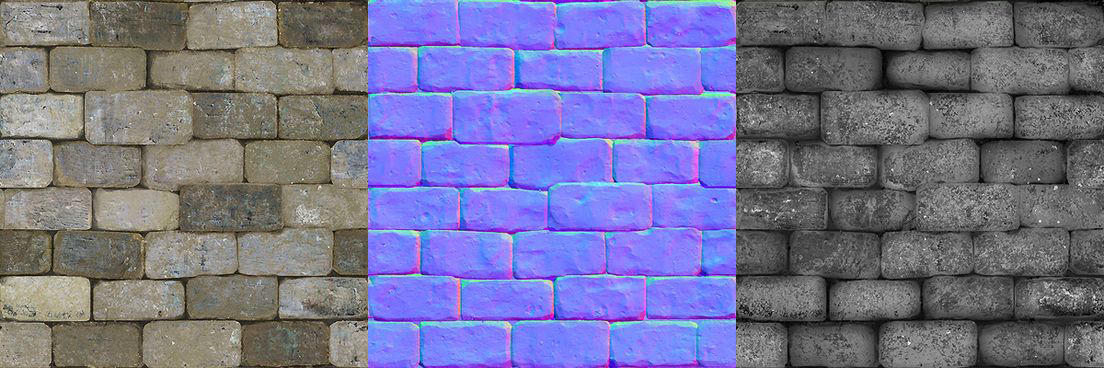
\includegraphics[width=0.8\textwidth]{images/brick_texture_maps.png}
    \caption{Diffúz, normál és spekuláris textúratérképek.}
\end{figure}

Számtalan, a normáltérképhez (\textit{normal map}) hasonló ,,trükkös'' textúrázás létezik még. Az elkészített megjelenítő a felület alapszínét jelentő diffúz értékeken kívül kívül Blinn-Phong árnyalás esetén az ambiens színt és a spekuláris tükröződési állandót, fizikai alapú árnyalás esetén pedig a rücskösség és fémesség értékeket képes textúrából olvasni. PBR esetén különösen látványos a textúrázás hatása: a mellékelt fegyver modellen jól megfigyelhető a változó rücskösség által okozott tükröződés-elmosódás, illetve a fém és szigetelő részeken eltérő spekuláris csillanás.

\subsection{Nagy dinamikatartományú megjelenítés}

A jelenleg elterjedt kijelzők túlnyomó többsége 24 bites RGB bemenet alapján dolgozik. Ez azt jelenti, hogy a képernyőn látható színek vörös, zöld és kék komponensekből állnak, ahol minden komponensre \(2^8\) bit jut, azaz 256 különböző értéket vehetnek fel. Elméletben tehát \((2^8)^3\), azaz körülbelül 16,7 millió különböző színt tudunk megjeleníteni. A valóságban ténylegesen megjelenített színmennyiség a kijelzők különböző fizikai paramétereitől függően változik, de az emberi szem csupán körülbelül 10 millió színt képes megkülönböztetni egymástól~\cite{judd1975color}, így ebben a tekintetben a technológia az emberi érzékelés előtt áll.

Van azonban egy másik nagyon fontos, megjelenítőt és érzékelőt egyaránt jellemző tulajdonság, a kontrasztarány, amit a legvilágosabb (fehér) és a legsötétebb (fekete) megjeleníteni/érzékelni képes szín közötti arányként definiálunk. Míg egy modern LCD kijelző a 24 bites színtér által meghatározott 256:1 bemenő kontrasztarányból kb. 1000:1 kimenő arányt tud megjeleníteni, addig az emberi szem különböző fényviszonyokhoz való rendkívül jó alkalmazkodóképességének köszönhetően ennél jóval nagyobb, kb. 1000:1 - 15000:1 kontrasztarány érzékelésére is képes.~\cite{human_eye_dynamic_range}

A nagy dinamikatartomány (\textit{high-dynamic-range, HDR}) fogalma először a fényképészet területén jelent meg. A probléma az volt --- illetve mind a mai napig az ---, hogy a fényképezőgépek felépítéséből adódóan egyetlen expozícióval nem lehet olyan képet készíteni, amely a teljes emberi szem által érzékelhető dinamikatartományt visszaadja. A fényképészek ezt úgy oldották meg, hogy az expozíciós időt --- és ezzel a bejövő fénymennyiséget --- változtatva több képet készítettek ugyanarról a jelenetről, majd egy végső lépésben (amelyet színleképezésnek [\textit{tone mapping}] hívnak) ezeket egy meghatározott metodika alapján egy képpé kombinálták. A fényképészet a dinamikatartományt ún. expozíciós értékkel (\textit{exposure value, EV}) méri, ahol EV eggyel való növekedése a beérkező fénymennyiség megkétszereződését jelenti.

\begin{figure}[!ht]
    \centering
    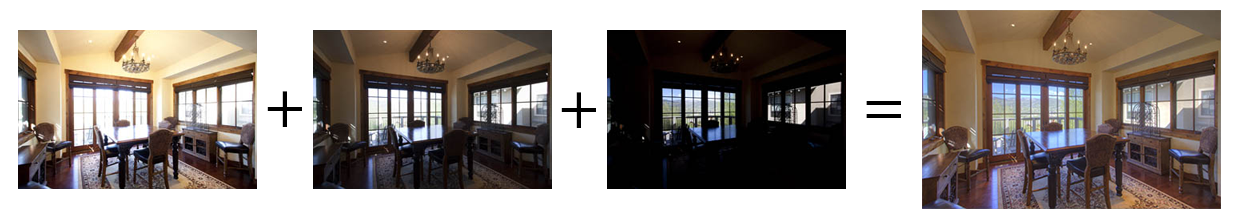
\includegraphics[width=1.0\textwidth]{images/hdr_process.png}
    \caption{HDR kép előállítása túl-, semlegesen és alulexponált fotókból.}
\end{figure}

Ahhoz tehát, hogy az általunk a valóságban érzékelhető fényerősség különbségeket érzékeltetni tudjuk, először is el kell szakadjunk az ebben minket korlátozó 24 bites színtértől. A modern grafikus kártyák már hardveresen támogatják a lebegőpontos (komponensenként 16 vagy 32 bites) puffereket, így ezeket használhatjuk HDR megjelenítésre. A fényképészettel ellentétben továbbra is csak egy leképezési lépésre van szükségünk, amely során egy ilyen lebegőpontos pufferbe számolunk, amelyben a korábbi maximális 255-nél fényerősségtől függően jóval nagyobb értékek is szerepelhetnek. A kijelzők azonban továbbra is a 24 bites, alacsony dinamikatartományú RGB színtérben várják a bemenetet, ezért HDR megjelenítésnél is szükség van egy színleképezési lépésre, amely során egy ún. színleképezési operátor segítségével a pufferben szereplő értékeket ismét ,,beszorítjuk'' a \([0; 1]\) intervallumba. Színleképezés során az alapvető cél az eredeti HDR kép lokális kontrasztarányainak minél jobb megtartása. Több ilyen operátor létezik, az egyik legegyszerűbb ezek közül a Reinhard operátor~\cite{reinhard2002photographic}:

\[
L_{ldr}(x, y) = { L_{hdr}(x, y) \over 1 + L_{hdr}(x, y) }
\]

ahol \(L_{hdr}(x, y)\) a (kétdimenziós) HDR puffer \((x, y)\) koordinátájában található érték.

Az elkészített megjelenítő három választható színleképezési operátort tartalmaz, amelyek megvalósítása a tone\_map.fs.glsl árnyalóban található. Az első az alapértelmezett Uncharted 2, amelyet készítői ,,filmszerűnek'' hívnak mozi-szerű színvilága miatt. Ezen kívül a fent említett Reinhard, illetve az Unreal Engine 4 alapértelmezett operátora került megvalósítása. Míg az előbbi igen fakó kimenetet ad, addig az utóbbi jelentősen megnöveli a színtelítettséget.

Nagy dinamikatartományú megjelenítéssel tehát jól modellezhetők a való világban tapasztalható fényviszonyok. Ugyanakkor egy új probléma is felmerül, mégpedig a fényviszonyokhoz történő adaptáció. Amikor például egy sötét szobából hirtelen kilépünk egy napsütötte teraszra, a szemünk --- bizonyítva rendkívüli alkalmazkodóképességét --- alkalmazkodik a hirtelen megváltozott fényerőhöz, pupillánk összeszűkül, hiszen a megnövekedett fénysűrűség miatt elég kisebb területen mintát vennie a színek megállapításához. Ezen effektus megvalósítása szinte kötelező egy HDR megjelenítő esetén, ugyanis hiába használunk nagy dinamikatartományt, enélkül a kevéssé vagy erősen megvilágított jelenetek természetellenesen sötétnek vagy világosnak hatnának.

A megvalósításhoz szükségünk van a jelenet átlagos fénysűrűségére, amely Erik Reinhard módszerével~\cite{reinhard2002photographic} a következőképpen számolható:

\[
L_{avg} = exp\left( { 1 \over N } \displaystyle\sum_{x, y} log(\delta + L_{rel}(x, y)) \right)
\]

\noindent
ahol

\begin{itemize}[noitemsep]
\item \(N\) a HDR puffer képpontjainak száma,
\item \(\delta\) egy kis érték \(log(0)\) elkerülésére abban az esetben, ha van fekete pixel a pufferben,
\item \(L_{rel}\) pedig a puffer \((x, y)\) pontjában vett relatív fényerősség.
\end{itemize}

Ennek implementációja az average\_luminance.fs.glsl árnyalóban található, lépései a következők: először egy \(64 \times 64\)-es textúrába számoljuk ki a logaritmus komponens értékeit, majd ezt egyszerű átlagszámítással csökkentjük előbb \(16 \times 16\)-os, majd \(4 \times 4\)-es és végül \(1 \times 1\)-es méretűre. Utolsó lépésként ezen az egy értéken a természetes alapú hatványt elvégezve kapjuk \(L_{avg}\)-t. Az első lépéshez szükségünk van a relatív fényerősségre, amely egy \([0; 1]\) intervallumba eső érték. RGB színtér esetén háromelemű színvektorral dolgozunk, ebből triviálisan átlagot számolva (\( { R + G + B } \over 3 \)) kaphatunk ilyen értéket. Szemünk viszont nem egyformán érzékeli a három alapszínt: az ún. fényerősség függvény (\textit{luminosity function}) alapján a zöld színre sokkal érzékenyebbek vagyunk, mint a vörösre vagy a kékre. Ezt figyelembe véve a fényerősség függvény és az azon alapuló sRGB konverzióból~\cite{stokes2012standard} származó konstans fényerősség vektor segítségével a következőképpen számolhatjuk a relatív fényerősséget:

\[
L_{rel} = [0.2126, 0.7152, 0.0722] \cdot L_{hdr}
\]

Mivel a színleképezés expozíció alapján működik, ezért az átlagos fénysűrűségből ezt valahogyan ki kell számoljuk. A DICE prezentációja~\cite{dice_moving_frostbite_to_pbr} alapján:

\[
EV = log_2\left({ L_{avg} \cdot S } \over K\right)
\]

\noindent
ahol

\begin{itemize}[noitemsep]
\item \(S\) a kamera ISO értéke,
\item \(K\) pedig egy eszközfüggő kalibrációs állandó.
\end{itemize}

Ebből látható, hogy az expozíciós érték definíciója függ az ISO értéktől. Mivel a mi esetünkben \(EV\)-t fénymennyiség mérésére használjuk, ezért az ISO-t 100-ban rögzítjük, és ezentúl \(EV_{100}\)-ként hivatkozunk rá. A \(K\) állandó értékét az ISO 2720:1974 szabvány 10,6 és 13,4 között javasolja meghatározni. Én --- a legtöbb modern 3D megjelenítőhöz hasonlóan --- 12,5-nek választottam, így

\[
EV_{100} = log_2\left({ L_{avg} \cdot 100 } \over 12,5\right)
\]

\noindent
Az expozíció ebből a DICE prezentációja alapján a következőképpen számolható:

\[
exposition = { 1 \over { 1,2 \cdot 2^{EV_{100}} } } = { 1 \over { 9,6 \cdot L_{avg} } }
\]

A színleképezés bemenetét képező \(L_{hdr}\) vektort ezzel az expozícióval megszorozva a fényerő-adaptáció működésbe lép.

A valóban élethű fényerősség adaptációhoz még egy dolog szükséges: a késleltetés. Szemünk ugyanis nem azonnal, hanem a változás mértékével arányosan lassan, fokozatosan alkalmazkodik a megváltozott fényviszonyokhoz. Ehhez el kell tároljuk a legutóbbi képkoca kirajzolása során mért átlagos fénysűrűséget, így a legutóbbi és az éppen kirajzolt állapot között az eltelt idő függvényében interpolációval kiszámolható az adaptáció aktuális mértéke, ezáltal szemünkhöz hasonlóan lassítva a folyamatot. Az adaptáció implementációja a luminance\_adapter.fs.glsl árnyalóban található, a használt interpoláció pedig a következő:

\[
L_{cur} = L_{prev} + (L_{avg} - L_{prev}) \cdot (1 - 0,98^{S_a \cdot t_{\delta}})
\]

\noindent
ahol

\begin{itemize}[noitemsep]
\item \(L_{prev}\) az előző képkocka kirajzolása során mért átlagos fénysűrűség,
\item \(L_{avg}\) az aktuális képkoca átlagos fénysűrűsége,
\item \(S_a\) állandó, amellyel az adaptáció sebessége szabályozható,
\item \(t_{\delta}\) az előző képkocka kirajzolása óta eltelt idő.
\end{itemize}

Az \(S_a\) állandónak az implementációban 60-as értéket adtam, ezzel a szemünkhöz hasonló gyorsasággal történik az adaptáció. Az eltelt idővel való szorzás azért szükséges, hogy ezzel függetlenítsük az algoritmust (az adaptáció sebességét) a kirajzolás sebességétől.

\subsection{Pont és zseblámpa fények}

A valóságban szinte mindig érkezik valamilyen fény a szemünkbe, még a legsötétebb éjszakákon is. Az aggteleki Baradla-barlangot végigjáró turistacsoportoknak a túravezetők előszeretettel mutatják meg, milyen az abszolút sötétség: a túra egy pontján a fényképezők, telefonok kikapcsolása után a mesterséges barlangi világítást is lekapcsolják. A számítógépes megjelenítésben ez a kiindulópont. Ahhoz, hogy egy jelenetből lássunk is valamit, szükségünk van legalább egy fényforrásra.

Valósidejű grafikában az igaziakat jól közelítő, de a valóságban nem létező, absztrakt fényforrásokat használunk, mert ezekkel könnyen és gyorsan tudunk számolni. A legegyszerűbb ilyen fényforrások a pont fények, amelyek egy pozícióval és intenzitással adottak. Mivel nincs területük, a sugárzást nem tudjuk értelmezni rajtuk. A sugárzási teljesítményt viszont fel tudjuk írni a sugárzási intenzitás segítségével, ha a pont fény körüli egységgömbön integrált számítunk:

\[
\phi = \int_S { I d\omega } = I \int_0^{2\pi} { \int_0^\pi { sin\theta d\theta d\Phi } } = I 4\pi
\]

ahol S a pont fény körüli egységgömb.

\vspace{12pt}
\noindent
A ~\ref{subsec:matbase} fejezetben megadott képletek alapján:

\[
E = { { d\phi } \over { dA } } = I { { d\omega } \over { dA } } = I { { cos\theta } \over { dist }^2 }
\]

\noindent
Ebből pedig már

\[
L_{out}(\mathbf{v}) = f_r(\mathbf{l}, \mathbf{v}) E = f_r(\mathbf{l}, \mathbf{v}) {}
\]

következik.

Ez lényegében az ún. inverz négyzet törvény, azaz a besugárzott teljesítmény a fényforrástól való távolság négyzetével csökken. Gyakorlati megvalósítás szempontjából problémát jelent, hogy ez alapján \(L_{out}\) sosem éri el a 0-t, azaz elesünk egy fontos optimalizációs lehetőségtől, a nem látható fények kivágásától. Ezért egy halványítási tényezőt is bevezetünk az árnyalóban:

\[
attenuation = { I \over {dist}^2 } max(0, 1 - { dist \over r })
\]

ahol \(dist\) a fényforrástól való távolság, \(r\) pedig egy sugár, amin kívül a pontfény hatását nem vesszük figyelembe.

A zseblámpa fényeknek (\textit{spot light}) pozíción és intenzitáson kívül iránya és nyitási szöge is van. Pontszerű mivolta miatt itt sem értelmezhető a sugárzás, de a pontfényekhez hasonló módon, csak gömb helyett kúpon véve az integrált a sugárzási teljesítmény kiszámolható:

\[
\phi = I \int_0^{2\pi} { \int_0^\theta { sin\theta d\theta d\Phi } } = I 2\pi (1 - cos\theta)
\]

ahol \(\theta\) a zseblámpa (külső) nyitási félszöge. A valódi zseblámpák fényéhez hasonló, a kivetített fénykör széléhez közeledve történő elhalványulást egy új paraméter felvételével szimulálhatjuk. Ezt a paramétert belső nyitási félszögnek nevezzük, ami legfeljebb \(\theta\) lehet. A belső és nyitási félszög között fokozatosan elhalványítjuk a lámpa fényét.

A pont és zseblámpa fények megvalósítása a direct\_lighting.fs.glsl árnyalóban található.

\subsection{Kép alapú megvilágítás}

A kép alapú megvilágítás egy gyakran használt módszer a globális megvilágítás szimulálására. Globális megvilágításnak azokat a fényeket hívjuk, amelyek egy adott felületet indirekt módon (valahonnan már egyszer visszaverődve) érnek. Kép alapú megvilágításnál kicsit tovább megyünk ennél, és egy előre elkészített textúrából olvassuk ki a felület adott pontját érő összes sugárzást.

Az elkészült program a megjelenített modell környezetét környezeti térképezéssel (\textit{environment mapping}), egy ún. skybox (,,égdoboz'') segítségével szimulálja. Ezt úgy kell elképzelni, mintha egy végtelen nagyságú kocka közepére állnánk, és ezen kocka belső oldallapjaira felfestenénk, amit az adott oldal középpontjára merőlegesen nézve látunk a köryezetünkből. A program a skybox.vs.glsl árnyaló segítségével transzformálja úgy a kocka csúcspontjait, hogy azok a nézeti pozíciótól függetlenek legyenek. A skybox.fs.glsl-ben pedig egy egyszerű textúraolvasással rajzoljuk ki a kocka oldalait. Ez a textúra viszont speciális, kockatérkép (\textit{cube map} típusú, amit a program Radiance HDR típusú nagy dinamikatartományú képekből olvas, amelyben függőleges kereszt elrendezésben találhatóak a kocka oldallapjainak textúrái.

Kép alapú megvilágítás esetén ebből a kockatérképből szeretnénk a megvilágítást kiszámolni. Pont és zseblámpa fények esetén könnyű dolgunk volt, hiszen a kimenő sugárzás kiszámolására használt integrálnak volt analitikus megoldása. Kép alapú megvilágításnál viszont a felület rücskössége miatt nem tudunk analitikus megoldást adni, az integrál értékét ezért valamilyen numerikus módszerrel kell közelítenünk. Az egyik legelterjedtebb ilyen módszer a Monte-Carlo integrálás. Ennek során az integrálandó függvényből \(N\) mintát veszünk, ezeket a mintákat elosztjuk egy valószínűségi sűrűségfüggvénnyel (\textit{probability density function, PDF}), majd összeadjuk őket:

\[
L_{out}(\mathbf{v}) = \int_{\Omega} { f_r(\mathbf{l}, \mathbf{v}) L_{in}(\mathbf{l})(-\mathbf{l} \cdot \mathbf{n}) d\mathbf{l} } \approx { 1 \over N } \sum_{k=1}^{N} { { f_r(\mathbf{l}, \mathbf{v}) L_{in}(\mathbf{l})(-\mathbf{l} \cdot \mathbf{n}) d\mathbf{l} } \over { p_r(\mathbf{v}, \mathbf{l}_k) } }
\]

Itt \(p_r\) az \(\mathbf{l}_k\) sűrűségfüggvénye. Egyenletes eloszlás esetén \(p_r = \frac{1}{2\pi}\), hiszen félgömbön integrálunk. A Monte-Carlo integrálás többféle mintavételezéssel is használható. A fent leírt egyenlet ezek közül a számítógépes grafikában gyakran használt fontosság szerinti mintavételezést alkalmazza.

Sugárkövetésen alapuló megjelenítőkhöz már felhasználhatóak ezek a képletek, valósidejű megjelenítéshez azonban a fontosság szerinti mintavételezés ellenére is túl nagy számításigényűek: a rücskösség növelésével egyre több mintát kellene vennünk. Ezért a kép alapú megvilágítást az Unreal Engine 4-ben használt technikával~\cite{karis2013real} valósítottam meg, aminek segítségével a besugárzás és a BRDF speciális textúrákba előre kiszámolható, és az \(\mathbf{n} = \mathbf{v} = \mathbf{l}\) feltételezésen alapszik:

\[
{ 1 \over N } \sum_{k=1}^{N} { { f_r(\mathbf{l}, \mathbf{v}) L_{in}(\mathbf{l})(-\mathbf{l} \cdot \mathbf{n}) d\mathbf{l} } \over { p_r(\mathbf{v}, \mathbf{l}_k) } } \approx
\]
\[
\approx { { 1 \over \sum_{k=1}^{N} cos{\theta_l}_k } \sum_{k=1}^{N} L_{in}(\mathbf{l}_k)cos{\theta_l}_k } + { 1 \over N \sum_{k=1}^{N} { { f_r(\mathbf{v}, \mathbf{l}_k) cos{\theta_l}_k} \over { p_r(\mathbf{v}, \mathbf{l}_k) } } }
\]

Az első tagot a rücskösség értékétől függően egy kockatérkép mip-map szintjeibe számolhatjuk ki. Ezt a textúrát besugárzási kockatérképnek hívjuk. A második tag egy ún. lookup textúrába számolható, azonban jelenleg 3 paramétertől (\(F_0\), rücskösség, \(\mathbf{n} \cdot \mathbf{v}\)) függ, így további egyszerűsítésre van szükség:

\[
\int_{\Omega} { f_r(\mathbf{l}, \mathbf{v}) cos\theta_l d\mathbf{l} } =
\]
\[= F_0 \int_{\Omega} { { f_r(\mathbf{l}, \mathbf{v}) \over F(\mathbf{v}, \mathbf{h}) } (1 - (1 - \mathbf{v} \cdot \mathbf{h})^5) cos\theta_l d\mathbf{l} } + \int_{\Omega} { { f_r(\mathbf{l}, \mathbf{v}) \over F(\mathbf{v}, \mathbf{h}) } (1 - \mathbf{v} \cdot \mathbf{h})^5 cos\theta_l d\mathbf{l} }
\]

\vspace{5pt}

Ezzel az \(F_0\)-tól való függést megszüntettük, és a két integrál értéke a kétdimenziós lookup textúra vörös és zöld csatornájában tárolható.

Mindezek segítségével valósidőben, mindössze két textúraolvasással kiszámolható a kép alapú megvilágításból származó sugárzás. Sőt, a két besugárzási kockatérképet (diffúz és spekuláris) és a BRDF lookup textúrát nem muszáj előre kiszámolni, dinamikus tükröződés megvalósításához kevesebb mintával menet közben is generálhatók. Az \(\mathbf{n} = \mathbf{v} = \mathbf{l}\) feltételezés azonban szemmel látható hibákat okoz: elsősorban sík felületeknél észrevehető, hogy a valóságban ,,megnyúlt'' tükröződések emiatt itt nem jelennek meg.

\section{Továbbfejlesztési lehetőségek}
\label{sec:further_dev}

Az elkészült megjelenítő ugyan alkalmas a fizikai alapú megjelenítés bemutatására, de számtalan lehetőség van a továbbfejlesztésre mind a felhasználói felület, mind a fizikai alapú megvilágítás szempontjából.

A felhasználói felületen hasznos lenne az anyagtulajdonságoknál a textúrabetöltés, ill. textúra előnézet lehetősége. Ezzel akár modellezők számára is hasznossá válna a program, egy modell elkészítése során ugyanis nagy segítséget jelentene, ha menet közben lehetne textúrát váltani, továbbá egy kis előnézeti kép is megjelenne róla. Ezen kívül a kamerakezelésen lehetne fejleszteni, például a nézet középpontjának egér jobb gombjával történő áthelyezése szabadabbá tenné a jelentben való mozgást.

A megjelenítő jelenleg egyetlen modellformátumot képes betölteni. Ezen például a tinyobjloader Assimp nyílt forráskódú modellbetöltő könyvtárra cserélésével lehetne változtatni --- az Assimp szinte az összes létező formátum betöltésére képes, illetve exportálási lehetőséget is tartalmaz. A skybox alapjául szolgáló HDR panorámaképek betöltését flexibilisebbé lehetne tenni, hogy ne csak függőleges kereszt, hanem más (pl. gömbtérképes) elrendezésű képeket is be tudjunk tölteni.

A fizikai alapú megjelenítés nem merül ki a kép alapú megvilágításban illetve a pont és zseblámpa fényeknél: a fejlett PBR-alapú megjelenítők gömb, kapszula (a két végén félgömbbel lezárt henger) és területi (síkbeli poligon) típusú fényforrások kezelésére is képesek. Ezek fizikai alapú, valósidőben történő megjelenítése aktív kutatási terület, a jelenleg használt közelítések nem teljesen korrektek, bizonyos tulajdonságokat (pl. energiamegmaradás) nem mindig teljesítenek. Az emberi szem meggyőzésére azonban már most is alkalmasak, ezért ezen fényforrások az aktuálisan használt közelítésekkel történő implementálása látványos eredményt hozna.

\textit{Megjegyzés: az aktív kutatási terület aktualitását mi sem bizonyítja jobban, hogy a szakdolgozat írása alatt jelent meg egy új, viszonylag kis számításigényű módszer a területi fények közelítésére~\cite{real_time_area_light}. }

Az elkészült megjelenítő az ún. \textit{forward rendering} technikát használja, aminek nagy hátránya, hogy egy képpont árnyalását minden egyes dinamikus fényre külön el kell végezni, azaz minden egyes dinamikus fényforráshoz újra ki kell rajzolni a jelenetet. Ezen lehetne segíteni például azzal, hogy nem az egész jelenetet, csak azokat a részeket árnyaljuk újra, amelyekre az adott fényforrás hatással van. Dinamikus fények megjelenítése szempontjából a legtöbbet azonban a \textit{deferred rendering} (késleltetett árnyalás) technikával lehetne nyerni: ezen módszer lényege, hogy egy speciális, G-Buffernek nevezett pufferben tároljuk a képpontok árnyalásához szükséges összes információt, így a fényforrások számától függetlenül, egy lépésben elvégezhető az árnyalás.

Mind a forward, mind a deferred megjelenítés esetén külön lépésre lenne szükség az átlátszó felületek megjelenítéséhez, amit a megjelenítő jelenleg nem támogat. Ehhez először az anyagokat átlátszatlan és átlátszó csoportra kellene bontani, majd az átlátszatlanokat forward vagy deferred technikával kirajzolni, végül az átlátszóakat egy utolsó lépésben megfelelően beállított színkeverési móddal rárajzolni a meglévő képre. Tudnunk kell azonban, hogy ez csak alapszintű támogatást jelent: valósidejű grafikában a mai napig nagy kihívást jelentő probléma egymást átfedő átlátszó felületek sorrendfüggetlen megjelenítése (\textit{order-independent transparency}), a létező megoldások még túl nagy számításigényűek ahhoz, hogy komplex jelenetek megjelenítésénél használni tudjuk őket.

A tesztelés során felszínre került egy hiba a besugárzási textúrák előre generálása során: a nagy értékeket tartalmazó HDR kockatérképek esetén a generált spekuláris besugárzási textúra zajos lesz. Ennek oka, hogy nagy értékek mellett a fontosság szerinti mintavételezés során a képpontonkénti 2048 mintavétel már nem elegendő az integrál kis hibájú közelítéséhez. Triviális megoldásnak tűnik a mintavétel-szám növelése, azonban tudnunk kell, hogy az árnyalóprogramok viszonylag rövid futásidőre vannak kitalálva, és egy bizonyos időkeretet túllépve (jellemzően alig pár másodperc) a grafikus kártya meghajtóprogramja egyszerűen leállítja programunkat. Ennek kiküszöbölésére a kockatérképet fel lehetne bontani kisebb (ideális esetben az intenzitástól függő nagyságú) részekre, majd ezeken lefuttatni az árnyalóprogramot és végül ezekből összerakni az eredeti méretű textúrát. Ezzel kicselezhető a meghajtóprogram, de a generálás továbbra is sokáig fog tartani a mintavételezés magas száma miatt, ezért az egész előgenerálási folyamatot külön alkalmazásban lenne érdemes megvalósítani.

\section{Tesztelés}

Egy 3D megjelenítő tesztelésénél némileg el kell térnünk a manapság széles körben elterjedt automatikus egységtesztelés módszertanától. Ennek oka az, hogy a megjelenítő által előállított kimenet nem egy könnyen ellenőrizhető, másik helyes kimenettel egy az egyben összehasonlítható eredmény (pl. szöveg), hanem egy kép. Ugyan léteznek módszerek két kép objektív összehasonlítására, ha ilyen módszerhez folyamodunk, felmerül a kérdés, hogy mit tekintünk helyes megoldásnak, \textit{referenciának}? Egy, az iparág által fizikai alapú megjelenítők esetében használt módszer a valósidejű mellé egy ugyanazon bemenetet használó, szintén fizikai alapú, de sugárkövetésen alapuló megjelenítőt fejleszteni, amellyel aztán a valósidejű megjelenítéshez használt megoldások, közelítések helyessége ellenőrizhető. Fontos kiemelni, hogy itt sem számítógép általi, automatikus összehasonlításról van szó: azt a kimenetet tekintjük helyesnek, amely ,,ránézésre'' jónak, fizikailag plauzibilisnek tűnik. Mivel egy külön sugárkövetéses megjelenítő fejlesztése csupán a tesztelés céljából bőven túlmutat ezen szakdolgozat keretein, ezért a kimenet tesztelésénél a szememre hagyatkoztam, és referenciának egy neves PBR alapú eszközt, a Marmoset Toolbag 2-t használtam.

\subsection{Alapvető funkciók helyes működésének ellenőrzése}

Mielőtt rátérnénk a kimenet tesztelésére, fontos leellenőriznünk, hogy a felhasználói interakció során a program helyesen működik, véd az alapvető felhasználói hibák ellen, illetve a különböző bemeneteket jól kezeli. Ennek alapján a programot a következőkben leírt manuális tesztelésnek vetettem alá:

\vspace{10pt}

\begin{center}

  \begin{tabulary}{\textwidth}{L | C || L}
    \multicolumn{3}{l}{\textbf{Modell betöltés tesztelése}} \\
    \hline
    Nem megfelelő formátumú modell betöltése & \checkmark & \footnotesize{A megfelelő szűrés be van állítva a tallózó párbeszédablakban. Érvénytelen .obj fájl esetén semmi sem jelenik meg.} \\
    \hline
    Nagy méretű modell betöltése & \checkmark & \footnotesize{55 MB-os modellel tesztelve. A betöltési idő értelemszerűen a mérettel arányosan nő.} \\
    \hline
    Hivatkozott, de nem létező .mtl fájl & \checkmark & \footnotesize{Egy alapértelmezett anyag jön létre ilyen esetekben.} \\
    \hline
    Üres .mtl fájl & \checkmark & \footnotesize{Lásd fentebb.} \\
    \hline
    Üres .obj fájl & \checkmark & \footnotesize{} \\
    \hline
  \end{tabulary}

  \vspace{15pt}

  \begin{tabulary}{\textwidth}{L | C || L}
    \multicolumn{3}{l}{\textbf{Skybox betöltés tesztelése}} \\
    \hline
    Nem megfelelő formátumú skybox betöltése & \checkmark & \footnotesize{Nincs rá lehetőség, hiszen a megfelelő szűrés be van állítva a tallózó párbeszédablakban.} \\
    \hline
    Nem megfelelő méretű skybox betöltése & \checkmark & \footnotesize{A program hibaüzenetet ad.} \\
    \hline
    Érvénytelen HDR fájl betöltése & \checkmark & \footnotesize{A program hibaüzenetet ad.} \\
    \hline
    Nem megfelelő elrendezésű skybox betöltése & \checkmark & \footnotesize{Hibás méretű kép esetén hibaüzenet jelenik meg.} \\
    \hline
    Besugárzási és BRDF textúrák előállítása & \checkmark & \footnotesize{A program külön ellenőrzi a BRDF, diffúz és spekuláris besugárzási textúrák meglétét, ha bármelyikből hiányzik, azt újragenerálja.} \\
    \hline
    Nagy értékeket tartalmazó skyboxból történő előgenerálás & \xmark & \footnotesize{Lásd továbbfejlesztési lehetőségek (~\ref{sec:further_dev} fejezet, utolsó bekezdés).} \\
    \hline
  \end{tabulary}

  \vspace{15pt}

  \begin{tabulary}{\textwidth}{L | C || L}
    \multicolumn{3}{l}{\textbf{Megjelenítő beállításainak tesztelése}} \\
    \hline
    Vertikális szinkronizáció & \checkmark & \footnotesize{Bekapcsolva a megszokott 60 FPS-sel történik a megjelenítés, kikapcsolva ennél többel, ha képes rá a grafikus kártya.} \\
    \hline
    Színleképezés működése & \checkmark & \footnotesize{Mindegyik színleképezési operátor kiválasztható és megfelelően működik.} \\
    \hline
    Automatikus expozíció & \checkmark & \footnotesize{Működik, a fényerősség észrevehetően adaptálódik a fényviszonyokhoz.} \\
    \hline
    Expozíciós érték & \checkmark & \footnotesize{A csúszkát állítgatva változik a fényerősség.} \\
    \hline
    Modell forgatása & \checkmark & \footnotesize{A jelölőnégyzet segítségével a modell forgatása be/kikapcsolható.} \\
    \hline
    A támogatott MSAA mintaszám túllépése & \checkmark & \footnotesize{A program automatikusan a támogatott maximális mintaszámot használja ilyenkor, erről értesítést is ír a konzolra.} \\
    \hline
    Érvénytelen MSAA mintaszám megadása & \checkmark & \footnotesize{Ha a mintaszám nem kettő hatványa, akkor az élsimítás letiltásra kerül és a program értesítést is ír a konzolra.} \\
    \hline
  \end{tabulary}

  \vspace{15pt}

  \begin{tabulary}{\textwidth}{L | C || L}
    \multicolumn{3}{l}{\textbf{Modellinformációs ablak tesztelése}} \\
    \hline
    PBR ki/bekapcsolása & \checkmark & \footnotesize{A kapcsoló működik. Kikapcsolt állapotban Blinn-Phong árnyalással jelenik meg a modell.} \\
    \hline
    Alakzat választás & \checkmark & \footnotesize{A választógombbal lehet az alakzatok között váltani, az ablak tartalma megfelelően frissül.} \\
    \hline
    Alakzat kirajzolásának ki/bekapcsolása & \checkmark & \footnotesize{} \\
    \hline
  \end{tabulary}

  \vspace{15pt}

  \begin{tabulary}{\textwidth}{L | C || L}
    \multicolumn{3}{l}{\textbf{Megvilágítási beállítások tesztelése}} \\
    \hline
    Kép alapú megvilágítás ki/bekapcsolása & \checkmark & \footnotesize{A kapcsoló működik. Kikapcsolt állapotban a modellre csak a pont/zseblámpa fény hat.} \\
    \hline
    Pont/zseblámpa fény kapcsolása & \checkmark & \footnotesize{Mindkét fényforrást a megfelelő jelölőnégyzettel ki/be lehet kapcsolni.} \\
    \hline
    Pont/zseblámpa fény színének és teljesítményének beállítása & \checkmark & \footnotesize{Mindkét fényforrás esetén a szín és a teljesítmény szemmel láthatóan változik.} \\
    \hline
    Zseblámpa fény nyitási szögének beállítása & \checkmark & \footnotesize{A két félszög módosítására a program megfelelően reagál. A belső nyitási szög nem lehet nagyobb a külsőnél, a külső nyitási szög nem lehet kisebb a belsőnél.} \\
    \hline
  \end{tabulary}

  \vspace{15pt}

  \begin{tabulary}{\textwidth}{L | C || L}
    \multicolumn{3}{l}{\textbf{Blinn-Phong anyagbeállítások tesztelése}} \\
    \hline
    Anyag kiválasztása & \checkmark & \footnotesize{Az ablak tartalma megfelelően frissül.} \\
    \hline
    Diffúz szín/textúra beállítása & \checkmark & \footnotesize{Szemmel láthatóan jól működik.} \\
    \hline
    Normáltérképezés be/kikapcsolása & \xmark & \footnotesize{Nem tökéletes. Egyes normáltérképek elrontják a megvilágítást, míg mások jól működnek.} \\
    \hline
    Ambiens szín/textúra beállítása & \checkmark & \footnotesize{Az ambiens szín láthatóan hozzáadódik a visszavert színhez.} \\
    \hline
    Spekuláris szín/textúra beállítása & \checkmark & \footnotesize{A spekuláris szín erőssége határozza meg a visszaverődés koncentráltságát.} \\
    \hline
    Ragyogás beállítása & \checkmark & \footnotesize{A ragyogást növelve egyre kisebb és koncentráltabbá válik a spekuláris csillanás.} \\
    \hline
  \end{tabulary}

  \vspace{15pt}

  \begin{tabulary}{\textwidth}{L | C || L}
    \multicolumn{3}{l}{\textbf{Fizikai alapú anyagbeállítások tesztelése}} \\
    \hline
    Anyag kiválasztása & \checkmark & \footnotesize{Az ablak tartalma megfelelően frissül.} \\
    \hline
    Előre beállított anyag kiválasztása & \checkmark & \footnotesize{Előre beállított anyagot kiválasztva az anyagtulajdonságok frissülnek és tetszőlegesen módosíthatóak.} \\
    \hline
    Diffúz szín/textúra beállítása & \checkmark & \footnotesize{Szemmel láthatóan jól működik.} \\
    \hline
    Normáltérképezés be/kikapcsolása & \xmark & \footnotesize{Lásd a Blinn-Phong anyagbeállítások tesztelésénél.} \\
    \hline
    Rücskösség beállítása & \checkmark & \footnotesize{A csúszkával a rücskösséget állítva jól láthatóan, élethűen változik a modellen a fények tükröződésének elmosódottsága.} \\
    \hline
    Fémesség beállítása & \checkmark & \footnotesize{Szigetelőknél a diffúz szín sokkal jobban közrejátszik a spekuláris tükröződésben az eltérő törési mutató miatt.} \\
    \hline
  \end{tabulary}

\end{center}

\subsection{A kimenet ellenőrzése}

A kimenet tesztelését a bevezetésben leírtak alapján egy másik fizikai alapú megjelenítő segítségével végeztem. A Marmoset Toolbag 2 egy 3D művészek által közkedvelt eszköz, ami lényegében hasonló a szakdolgozat keretében elkészült megjelenítőhöz, csak jóval nagyobb tudású. Mivel ennek a tesztelésnek a szemmel történő összehasonlítás adja az alapját, így az mindegyik tesztesethez mellékeltem a két megjelenítő kimenetét.

\vspace{15pt}

\noindent
\textbf{Összetett modell tesztelése}

Ennél a tesztesetnél a mellékelt fegyver modell megjelenítését teszteltem, amely rendelkezik diffúz, rücskösségi és fémességi textúrával is, így jó alapot ad az összehasonlításra.

\begin{figure}[!ht]
    \centering
    \begin{subfigure}[b]{0.45\textwidth}
        \centering
        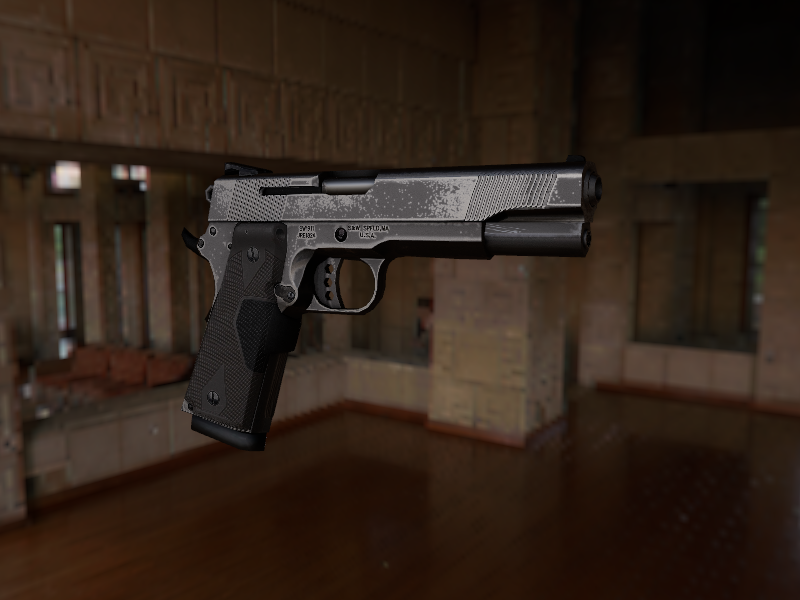
\includegraphics[width=\textwidth]{images/scr_ennis.png}
        \caption{Eredmény}
    \end{subfigure}
    \hfill
    \begin{subfigure}[b]{0.45\textwidth}
        \centering
        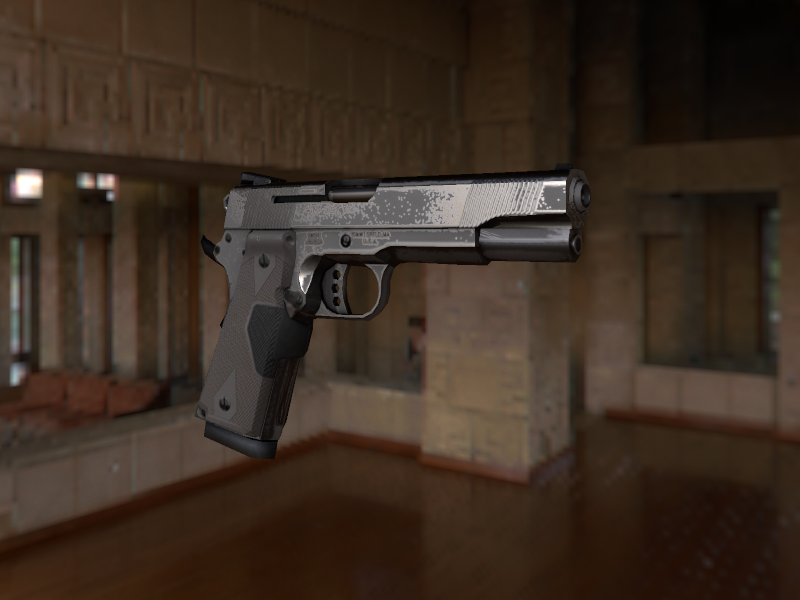
\includegraphics[width=\textwidth]{images/marmoset_ennis.png}
        \caption{Referencia}
    \end{subfigure}
\end{figure}

A képeken jól látható, hogy minimálisan eltérések vannak kamera pozícióban, modell elforgatásban és skybox fényerőben. Ennek oka az, hogy a két megjelenítőnek nem ugyanaz a bemenete: a Marmoset rendelkezik saját jelenetleíró fájllal, viszont az enyém nem, emiatt mindkét esetben kézzel kellett minden paramétert beállítani, ez pedig nyilvánvalóan kisebb eltéréseket okoz.

\textit{Eredmény:} a megjelenítő által előállított kép meggyőzően hasonlít a Marmoset által előállítottra. Az apró visszaverődési eltéréseket az előbb említett beállításbeli pontatlanságok okozzák.

\vspace{15pt}

\noindent
\textbf{Felületi rücskösség tesztelése}

Ennél a tesztesetnél a mellékelt gömb modell segítségével ellenőriztem, hogy a megjelenítő a különböző rücskösségi értékek alapján milyen kimenetet állít elő. Ehhez előbb 1-re (legsimább), majd 0,5-re, végül 0-ra (legdurvább) állítottam a rücskösség értékét. A gömb diffúz színét pirosra állítottam be, az anyagot szigetelőnek (0-s fémesség) definiáltam.

\begin{figure}[!ht]
    \centering
    \begin{subfigure}[b]{0.28\textwidth}
        \centering
        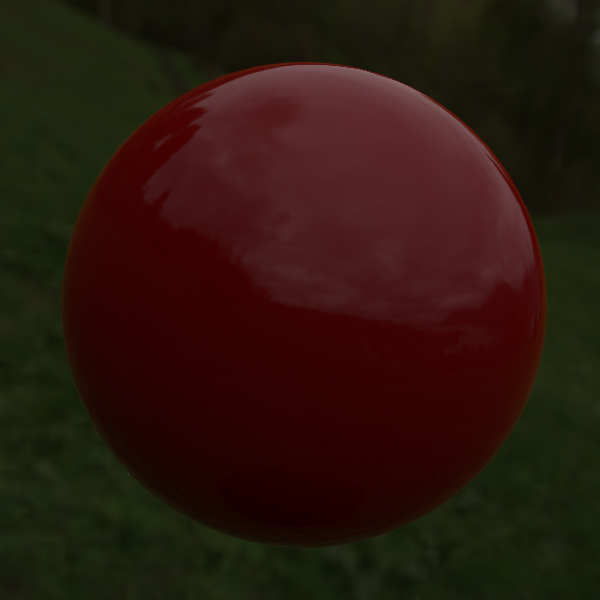
\includegraphics[width=\textwidth]{images/scr_r1.png}
        %\caption{Eredmény}
    \end{subfigure}
    \hfill
    \begin{subfigure}[b]{0.28\textwidth}
        \centering
        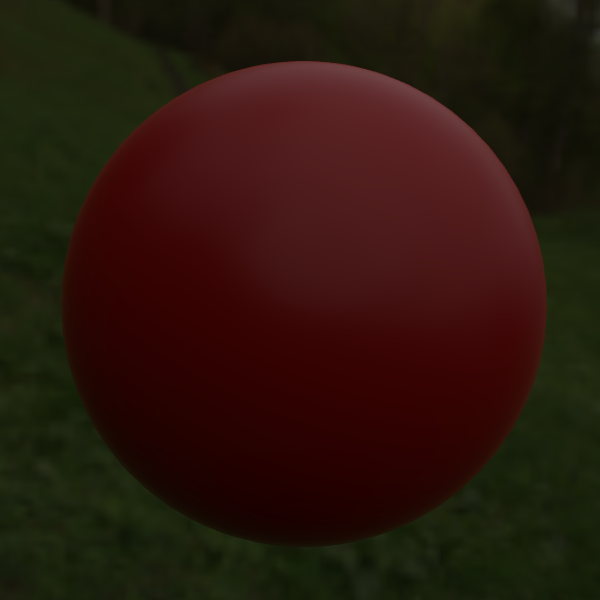
\includegraphics[width=\textwidth]{images/scr_r05.png}
        %\caption{Referencia}
    \end{subfigure}
    \hfill
    \begin{subfigure}[b]{0.28\textwidth}
        \centering
        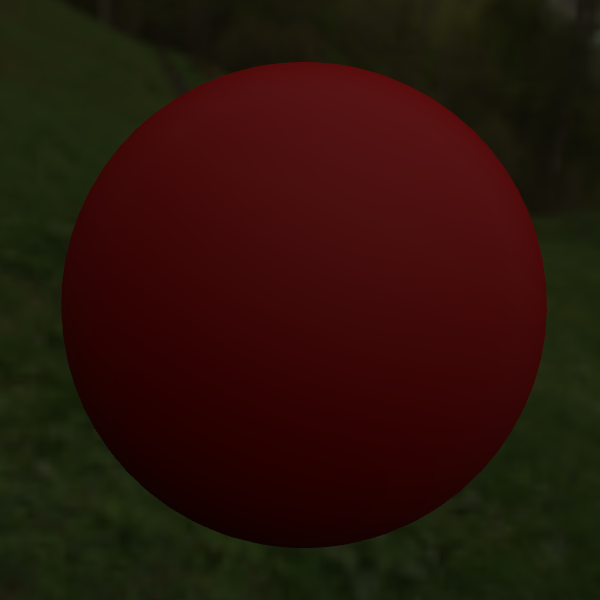
\includegraphics[width=\textwidth]{images/scr_r0.png}
        %\caption{Referencia}
    \end{subfigure}
    \caption{Eredmény}
\end{figure}

\begin{figure}[!ht]
    \centering
    \begin{subfigure}[b]{0.28\textwidth}
        \centering
        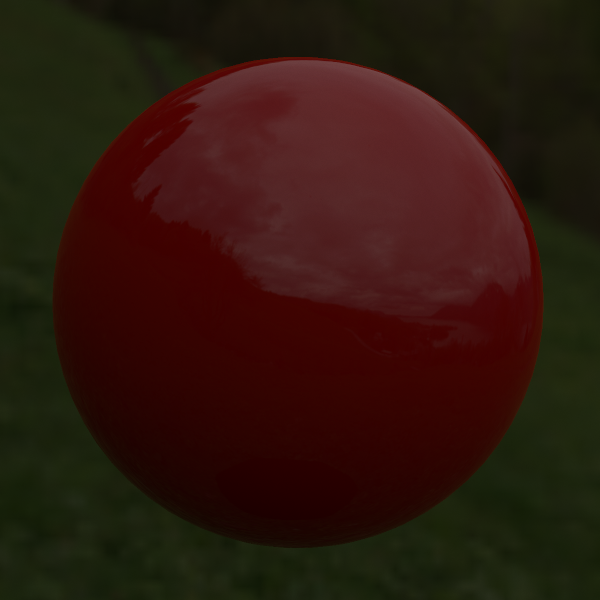
\includegraphics[width=\textwidth]{images/marmoset_r1.png}
        %\caption{Eredmény}
    \end{subfigure}
    \hfill
    \begin{subfigure}[b]{0.28\textwidth}
        \centering
        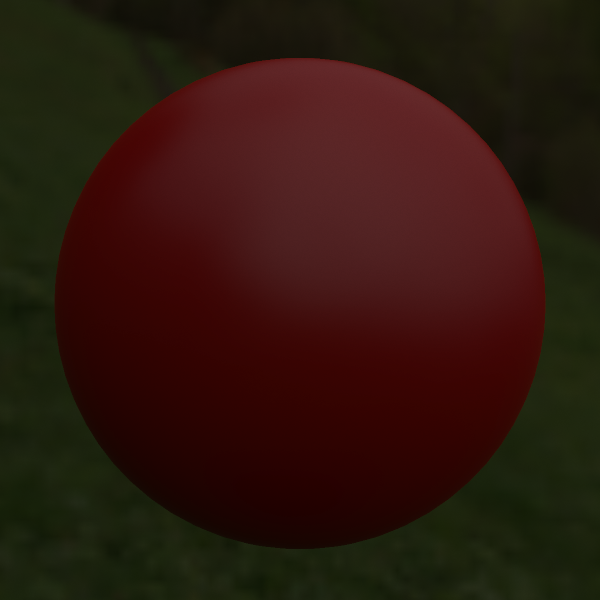
\includegraphics[width=\textwidth]{images/marmoset_r05.png}
        %\caption{Referencia}
    \end{subfigure}
    \hfill
    \begin{subfigure}[b]{0.28\textwidth}
        \centering
        
\includegraphics[width=\textwidth]{images/marmoset_r0.png}
        %\caption{Referencia}
    \end{subfigure}
    \caption{Referencia}
\end{figure}

\textit{Eredmény:} a két megjelenítő által előállított kép nagyon hasonlít egymásra. Apró különbségek csak a Fresnel-effektus mértékében mutatkoznak.

\vspace{15pt}

\noindent
\textbf{Fémesség tesztelése}

Szintén a mellékelt gömb modell segítségével teszteltem, hogy a megjelenítő milyen kimenetet ad fémes illetve szigetelő anyagok esetén. Ehhez előbb 1-re (fémes), majd 0-ra (nem fémes) állítottam a fémesség értékét. A felületi durvaságot 0,5-re állítottam, és a diffúz színt fehérnek választottam.

\begin{figure}[!ht]
    \centering
    \begin{subfigure}[b]{0.8\textwidth}
        \centering
        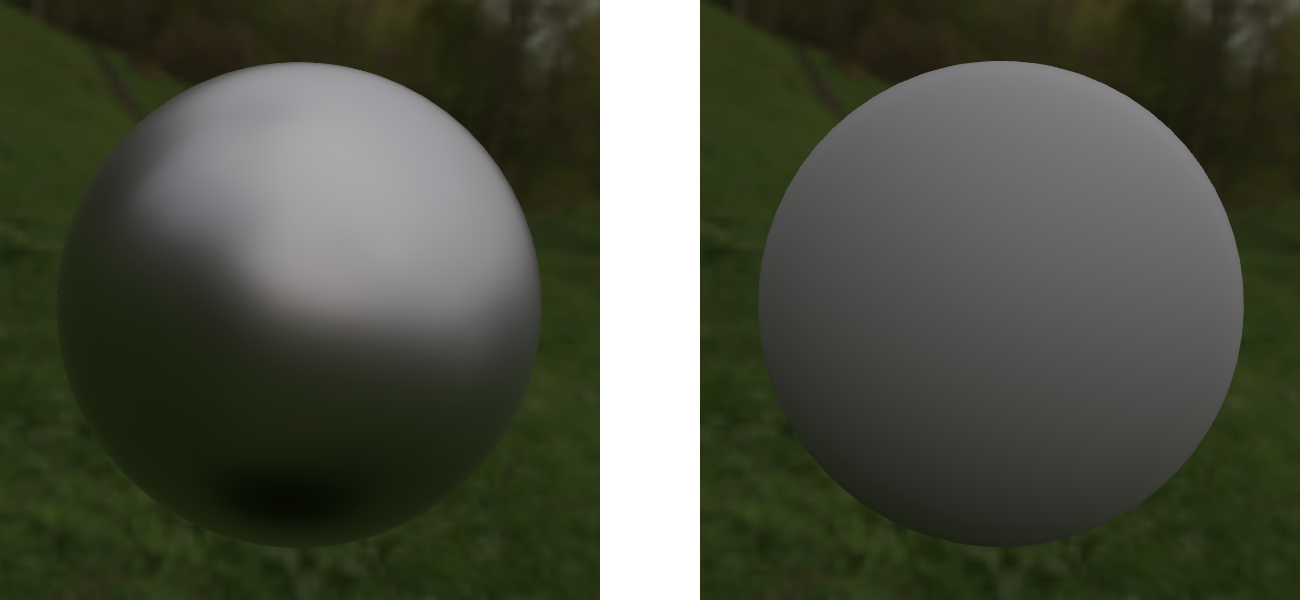
\includegraphics[width=\textwidth]{images/scr_metalness.png}
        %\caption{Eredmény}
    \end{subfigure}
    \caption{Eredmény}
\end{figure}

\begin{figure}[!ht]
    \centering
    \begin{subfigure}[b]{0.8\textwidth}
        \centering
        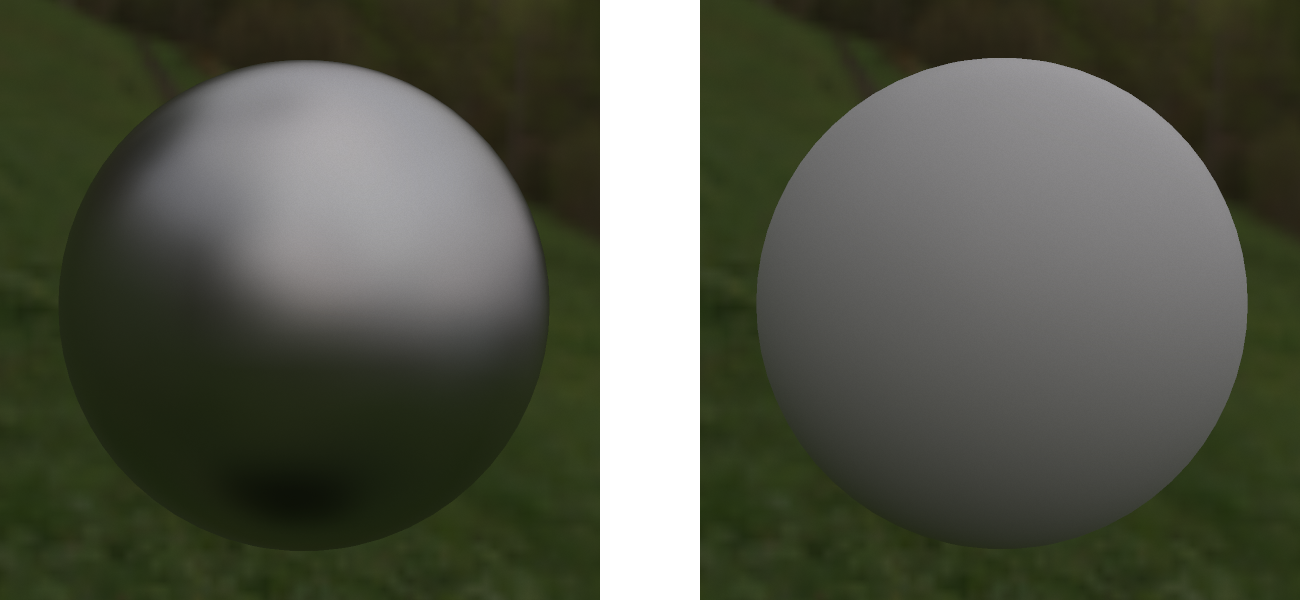
\includegraphics[width=\textwidth]{images/marmoset_metalness.png}
        %\caption{Eredmény}
    \end{subfigure}
    \caption{Referencia}
\end{figure}

\textit{Eredmény:} a két megjelenítő által előállított kép nagyon hasonlít egymásra. Apró különbségek csak a Fresnel-effektus mértékében mutatkoznak.

A kimenet tesztelése tehát összességében sikerrel zárult: az elkészült megjelenítő apróbb, elsősorban beállítási különbségekből fakadó eltérésekkel ugyan, de szemmel láthatóan szinte teljesen hasonló kimenetet ad, mint a szintén fizikai alapú, professzionális Marmoset Toolbag 2.

\bibliography{documentation}{}
\bibliographystyle{plain} 